% easychair.tex,v 3.4 2016/10/19

%\documentclass{easychair}
\documentclass[EPiC]{easychair}
%\documentclass[debug]{easychair}
%\documentclass[verbose]{easychair}
%\documentclass[notimes]{easychair}
%\documentclass[withtimes]{easychair}
%\documentclass[a4paper]{easychair}
%\documentclass[letterpaper]{easychair}
\usepackage[defaultlines=4,all]{nowidow}
\usepackage{doc}
\usepackage{subfigure}
\usepackage{tabularx}
\usepackage{booktabs}
\usepackage{framed}
%\usepackage{todonotes}

% GF: increasing penalties to avoid orphans and widows
\widowpenalty10000
\clubpenalty10000

%\usepackage{showframe}

% use this if you have a long article and want to create an index
% \usepackage{makeidx}

% In order to save space or manage large tables or figures in a
% landcape-like text, you can use the rotating and pdflscape
% packages. Uncomment the desired from the below.
%
% \usepackage{rotating}
% \usepackage{pdflscape}

% Some of our commands for this guide.
%
\newcommand{\easychair}{\textsf{easychair}}
\newcommand{\miktex}{MiK{\TeX}}
\newcommand{\texniccenter}{{\TeX}nicCenter}
\newcommand{\makefile}{\texttt{Makefile}}
\newcommand{\latexeditor}{LEd}

\newcommand{\ques}[1]{\textcolor{red}{#1}}

%\makeindex

%% Front Matter
%%
% Regular title as in the article class.
%
\title{ARCH-COMP19 Category Report:\\Continuous and Hybrid Systems with Nonlinear Dynamics}

% Authors are joined by \and. Their affiliations are given by \inst, which indexes
% into the list defined using \institute
%
\author{
 Fabian Immler\inst{1}
 \and
 Matthias Althoff\inst{2}
 \and
 Luis Benet \inst{3}
 \and
 Alexandre Chapoutot\inst{4}
 \and
 Xin Chen\inst{5}
\and
 Marcelo Forets \inst{6}
 \and
%  Goran Frehse\inst{4}
%  \and
 Luca Geretti\inst{7}
 \and
 Niklas Kochdumper\inst{2}
 \and
 David P. Sanders \inst{8}
 \and
 Christian Schilling \inst{9}
%  Yangge Li\inst{3}
%   \and
%  Sayan Mitra\inst{3}
%  \and
%  Mahendra Singh Tomar\inst{1}
%  \and
%  Majid Zamani\inst{1}
 }

\institute{
  Computer Science Department,
  Carnegie Mellon University, 
  United States\\
  \email{fimmler@cs.cmu.edu}\\
\and  
  Technische Universit\"at M\"unchen, 
  Munich, Germany\\
  \email{althoff@in.tum.de,niklas.kochdumper@tum.de}\\
\and  
  University of Dayton,
  Dayton, OH, United States\\
  \email{xchen4@udayton.edu}
% \and
%     University of Illinois at Urbana-Champaign,
%     Champaign, IL, United States\\
%     \email{\{mitras,cfan10,li213\}@illinois.edu}
\and
  ENSTA ParisTech,
   Palaiseau, France\\
   \email{\{alexandre.chapoutot,goran.frehse\}@ensta-paristech.fr}
\and
  University of Verona,
  Verona, Italy\\
  \email{luca.geretti@univr.it}
  \and
    Instituto de Ciencias F\'isicas, Universidad Nacional Aut\'onoma de M\'exico (UNAM), M\'exico\\
  \email{benet@icf.unam.mx}
  \and
    Universidad de la Rep\'ublica, Uruguay \\
    \email{mforets@gmail.com}
 \and
      Departamento de F\'isica, Facultad de Ciencias F\'isicas, \\ Universidad Nacional Aut\'onoma de M\'exico (UNAM), M\'exico\\
  \email{dpsanders@ciencias.unam.mx} \\
  \and
      IST Austria, Klosterneuburg, Austria  \\
  \email{christian.schilling@ist.ac.at}
}
\authorrunning{Immler \emph{et al.}}
\titlerunning{ARCH-COMP19 Nonlinear Dynamics}

\begin{document}

\maketitle

\newcommand{\toolnames}{Ariadne, CORA, DynIbex, Flow*, Isabelle/HOL, and JuliaReach}
\newcommand{\toolnumber}{6}

\begin{abstract}
 We present the results of a friendly competition for formal verification of continuous and hybrid systems with nonlinear continuous dynamics. The friendly competition took place as part of the workshop \underline{A}pplied Ve\underline{r}ification for \underline{C}ontinuous and \underline{H}ybrid Systems (ARCH) in 2019. In this year, \toolnumber{} tools \toolnames{} (in alphabetic order) participated. They are applied to solve reachability analysis problems on four benchmark problems, one of them with hybrid dynamics. We do not rank the tools based on the results, but show the current status and discover the potential advantages of different tools.
\end{abstract}

%\setcounter{tocdepth}{2}
%{\small
%\tableofcontents}

% GF: adding newpage to avoid the section header
%     being a lone orphan
\newpage
\section{Introduction}
\label{sect:introduction}

\begin{framed}
\paragraph{Disclaimer} The presented report of the ARCH friendly competition for \textit{continuous and hybrid systems with nonlinear dynamics} aims at providing a landscape of the current capabilities of verification tools. We would like to stress that each tool has unique strengths---not all of the specificities can be highlighted within a single report. To reach a consensus in what benchmarks are used, some compromises had to be made so that some tools may benefit more from the presented choice than others. The obtained results have been verified by an independent repeatability evaluation. To establish further trustworthiness of the results, the code with which the results have been obtained is publicly available as Docker~\cite{boettiger2015introduction} containers at \href{https://gitlab.com/goranf/ARCH-COMP}{gitlab.com/goranf/ARCH-COMP}.
\end{framed}


In this report, we summarize the results of the second ARCH friendly competition on the reachability analysis of continuous and hybrid systems with nonlinear dynamics. Given a system defined by a nonlinear Ordinary Differential Equation (ODE) $\dot{\vec{x}} = f(\vec{x},t)$ along with an initial condition $\vec{x} \in X_0$ as well as an unsafe set $U$, we apply the participating tools to prove that there is no state reachable contained in $U$ over a bounded time horizon. The techniques for solving such a problem are usually very sensitive to not only the nonlinearity of the dynamics but also the size of the initial set. This is also one of the main reasons why most of the tools require quite a lot of computational parameters.


In this report, \toolnumber{} tools \toolnames{} participate in solving the safety problems defined on three continuous and one hybrid benchmark. The continuous benchmarks are the Van der Pol oscillator, the Laub-Loomis model, and a controlled quadrotor model. The hybrid benchmark models a space rendezvous.

The benchmarks are selected based on the discussions of the tool authors. Since the experimental results are produced on different platforms, we provide Section~\ref{sec:machines} for the hardware details.



%------------------------------------------------------------------------------
\section{Participating Tools}
\label{sect:tools}

\paragraph{Ariadne.} (Luca Geretti) \textit{Ariadne} \cite{collins-adhs2012, benvenuti-ijrnc2014} is a library based on \textit{Computable Analysis} \cite{Weihrauch2000} that uses a rigorous numerical approach to all its algebraic, geometric and logical operations. In particular, it forces conservative rounding of all external and internal operations, in order to guarantee formal correctness of its results. It focuses on nonlinear systems, both continuous and hybrid, supporting differential and algebraic relations. It is written in C++ with growing support for a Python interface. The official site for Ariadne is \url{http://www.ariadne-cps.org}, while the version used for this competition is the development one available at \url{https://github.com/ariadne-cps/ariadne}.

\paragraph{CORA.} (Matthias Althoff, Niklas Kochdumper) The tool \textit{COntinuous Reachability Analyzer} (CORA) \cite{Althoff2015a, Althoff2016a} realizes techniques for reachability analysis with a special focus on developing scalable solutions for verifying hybrid systems with nonlinear continuous dynamics and/or nonlinear differential-algebraic equations. A further focus is on considering uncertain parameters and system inputs. Due to the modular design of CORA, much functionality can be used for other purposes that require resource-efficient representations of multi-dimensional sets and operations on them. CORA is implemented as an object-oriented MATLAB code. The modular design of CORA makes it possible to use the capabilities of the various set representations for other purposes besides reachability analysis. CORA is available at \url{http://www6.in.tum.de/Main/SoftwareCORA}.

% \paragraph{CORA/SX.} (Goran Frehse) CORA/SX is a port of the basic zonotope reachability algorithm from the CORA Matlab toolbox to SpaceEx. There are some differences between CORA and CORA/SX. We believe they have only a minor effect on the results in this report, and we will summarize them briefly. CORA/SX varies slightly in that some matrix computations (which approximate the input over one time step) use SpaceEx code instead of an overapproximation that is based on intervals. CORA/SX uses its own proprietary symbolic differentiation to compute the Jacobian and Hessian matrices. Affine arithmetic based on the library AAFlib \cite{grabowski2008analog} is used to obtain interval bounds on the linearization error.

 \paragraph{DynIbex.} (Alexandre Chapoutot) It is a library merging interval constraint satisfaction problem algorithms and guaranteed numerical integration methods based on Runge-Kutta numerical schemes implemented with affine arithmetic. This library is able to solve ordinary differential equations \cite{alexandreditsandretto:hal-01243053} and algebraic differential equations of index $1$ \cite{alexandreditsandretto:hal-01243044}, combined with numerical constraints on  state variables and reachable tubes. It produces sound results taking into account round-off error in floating-point computations and truncation errors generated by numerical integration methods \cite{doi:10.1080/10556788.2018.1459620}. 
 Moreover, constraint satisfaction problem algorithms offer a convenient approach to check properties on reachable tubes as explained in \cite{alexandreditsandretto:hal-01954764}. This library implements in a very generic way validated numerical integration methods based on Runge-Kutta methods without many optimizations. Indeed, the computation of the local truncation error, for each methods, depends only on the coefficients of Runge-Kutta methods and their order. DynIbex is freely available at \url{http://perso.ensta-paristech.fr/~chapoutot/dynibex/}. Figures have been produced with VIBes library \cite{Drevelle2014} which is available at \url{http://enstabretagnerobotics.github.io/VIBES/}.

% \paragraph{C2E2.}
% C2E2 (Compare-Execute-Check-Engine) \cite{c2e2_2,c2e2_1} is a tool for verifying bounded-time invariant properties for hybrid system with both linear or nonlinear dynamics,
% and discrete transitions with guards and resets. The tool implements a \textit{simulation-based approach} for overapproximating the reachable states. The input hybrid automata and the unsafe set has to be represented in an XML format. The new version of C2E2 used for these experiments (to be released in Fall 2018) comes with a model editor that can compose hybrid automata and a built-in plotter. C2E2 and related publications are available from~\url{https://publish.illinois.edu/c2e2-tool/}.


\paragraph{Flow*.} (Xin Chen) The tool Flow*~\cite{Chen+/2013/flowstar,Chen/2015/phd} uses an adapted Taylor Model (TM) integration method to compute reachable set overapproximations for nonlinear continuous and hybrid systems. Similar to the original method proposed in~\cite{Berz+Makino/1998/Verified}, an ODE solution, i.e., a function over the initial set as well as the time variable, over a bounded time interval is overapproximated by a TM in Flow*, and it therefore forms an overapproximation of the reachable set there. We also call this TM a TM flowpipe. For the discrete jumps of hybrid systems, Flow* uses the techniques of domain contraction and range overapproximation to compute flowpipe/guard intersections~\cite{Chen+/2012/taylor_models}, and then aggregates them by a box or parallelotope. Besides, in order to reduce the accumulation of overestimation during an integration job, the tool can symbolically represent the remainders of the previous $N$ flowpipes for some $N > 0$ (see~\cite{Chen+Sankaranarayanan/2016/decomposed}). In order to produce guaranteed results, the tool includes all roundoff errors in the TM remainders during reachability computation. This year, we entirely updated the module to handle continuous dynamics in Flow*, and all of the continuous benchmarks will be tested on it.



\paragraph{Isabelle/HOL-ODE-Numerics.}(Fabian Immler)
HOL-ODE-Numerics~\cite{Immler2015-TACAS,ODE-AFP} is a collection of rigorous numerical algorithms for continuous systems. It is based on Runge-Kutta methods implemented with affine arithmetic. 
The distinctive feature is that all algorithms are formally verified in the interactive
theorem prover Isabelle/HOL: everything from single roundoff errors to the global approximation
scheme is proved correct with respect to a formalization of ODEs in Isabelle/HOL.
The resulting code is therefore highly trustworthy.
It does, however, not feature many optimizations or the most sophisticated algorithms. We therefore
do not expect competitive performance figures. Nevertheless, the tool should exhibit reasonable
performance: it should scale (modulo possibly large constant factors) like ``regular'' tools
implementing similar algorithms. Isabelle/HOL is available at \url{https://isabelle.in.tum.de}, HOL-ODE-Numerics is part of the Archive of Formal Proofs \url{http://isa-afp.org/entries/Ordinary_Differential_Equations.shtml}.


\paragraph{JuliaReach.} (Marcelo Forets, Christian Schilling, David P. Sanders, Luis Benet) JuliaReach~\cite{BogomolovFFPS19} is a toolbox for reachability computations of dynamical systems, available at \url{http://juliareach.org}. For nonlinear reachability we combine functionality from \href{https://github.com/JuliaIntervals/TaylorModels.jl}{TaylorModels.jl}~\cite{TaylorModels.jl}, \href{https://github.com/JuliaDiff/TaylorSeries.jl}{TaylorSeries.jl}~\cite{TaylorSeries.jl} and \href{https://github.com/PerezHz/TaylorIntegration.jl}{TaylorIntegration.jl}~\cite{TaylorIntegration.jl}. First, we compute a non-validated integration using a Taylor model of order $n_T$. The coefficients of that series are polynomials of order $n_Q$ in the variables that denote the small variations of the initial conditions. We obtain a time step from the last two coefficients of this time series. In order to validate the integration step, we compute a second integration using intervals as coefficients of the polynomials in time, and we obtain a bound for the integration using a Lagrange-like remainder. The remainder is used to check the contraction of a Picard iteration. If the combination of the time step and the remainder do not satisfy the contraction, we iteratively enlarge the remainder or possibly shrink the time step. Finally, we evaluate the initial Taylor series with the valid remainder at the time step for which the contraction has been proved, which is also evaluated in the initial box of deviations from the central initial condition, to yield an over-approximation. The approach is (numerically) sound due to rigorous interval bounds in the Taylor approximation.
%------------------------------------------------------------------------------

\newpage

\section{Benchmarks}
\label{sect:benchmarks}

\subsection{Van der Pol Oscillator}

\subsubsection{Model}

The Van der Pol oscillator was introduced by the Dutch physicist Balthasar van der Pol. It can be defined by the following ODE with $2$ variables.
\[
 \left\{
 \begin{array}{lcl}
  \dot{x} & = & y \\
  \dot{y} & = & \mu(1 - x^2) y - x
 \end{array}
 \right.
\]
The system has a stable limit cycle however that becomes with increasingly sharp for higher values of $\mu$.

\subsubsection{Specification}
We consider $\mu = 1$ and $\mu = 2$.

\paragraph{$\mu = 1$:} For $\mu = 1$ we set the initial condition $x(0)\in [1.25,1.55]$, $y(0) \in [2.35,2.45]$, which was used in~\cite{Althoff/2010/phd}. The unsafe set is given by $y \geq 2.75$ for a time horizon of $[0, 7]$.

\paragraph{$\mu = 2$:} For $\mu = 2$ we set the initial condition $x(0)\in [1.55,1.85]$, $y(0) \in [2.35,2.45]$, which is the same size as before, but on the limit cycle for $\mu = 2$. The unsafe set is given by $y \geq 4.0$  for a time horizon of $[0, 8]$.


\subsubsection{Results}
We observe that $\mu = 2$ is harder for all of the tools.
Ariadne, DynIbex, Flow*, and JuliaReach deal with this difficulty by splitting the initial set (more). CORA and Isabelle/HOL introduce additional pseudo-invariants.
The time costs of the participating tools on the Van der Pol oscillator benchmark are given in Table~\ref{tab:compTimes:vanderpol}, and the plots of the overapproximation sets are presented in Figure~\ref{fig:vanderpol}. We also provide the computational settings of the tools as below.

\begin{figure}[p]
\centering
\subfigure[Ariadne.] 
	  {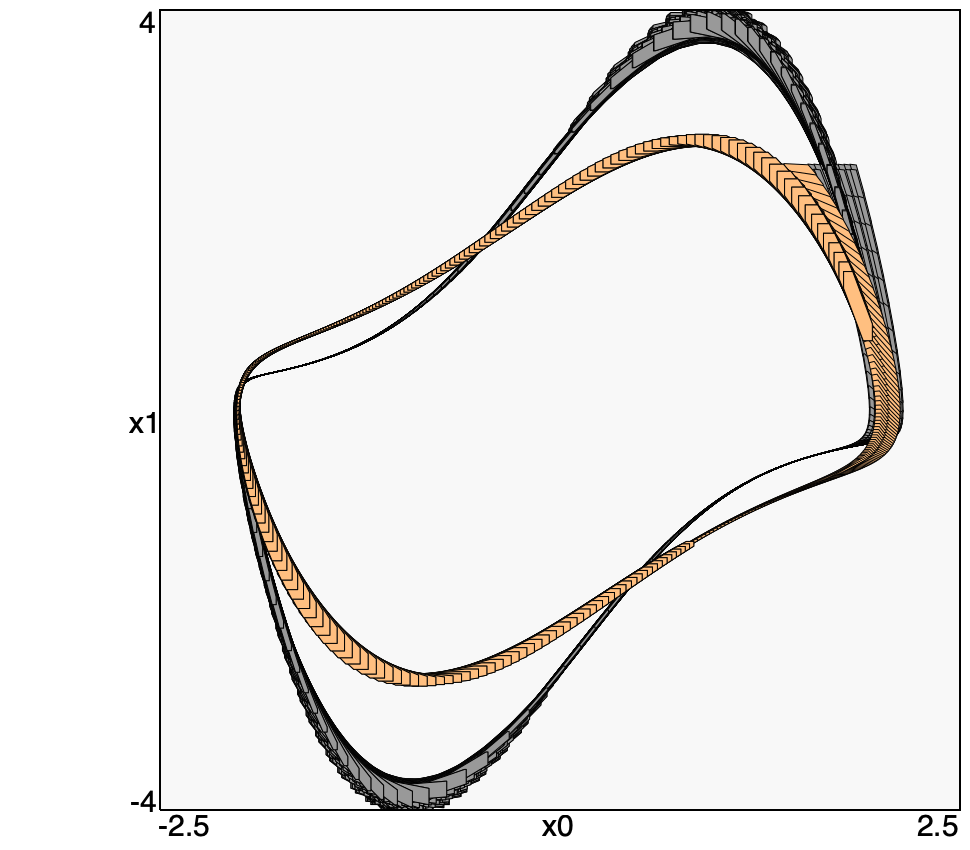
\includegraphics[width=5.5cm, height=5.0cm]{results_Ariadne/vanderpol.png}
  \label{fig:vanderpol:Ariadne}}
%  \hspace{0.2in}
\subfigure[CORA.] 
	  {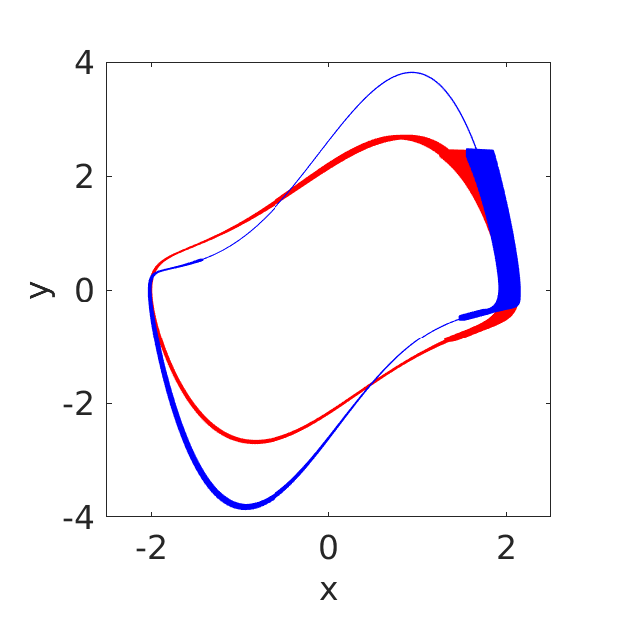
\includegraphics[width=5.5cm, height=5.5cm]{results_CORA/vanDerPol_27March2019.eps}
  \label{fig:vanderpol:CORA}}
  \subfigure[DynIbex.] 
	  {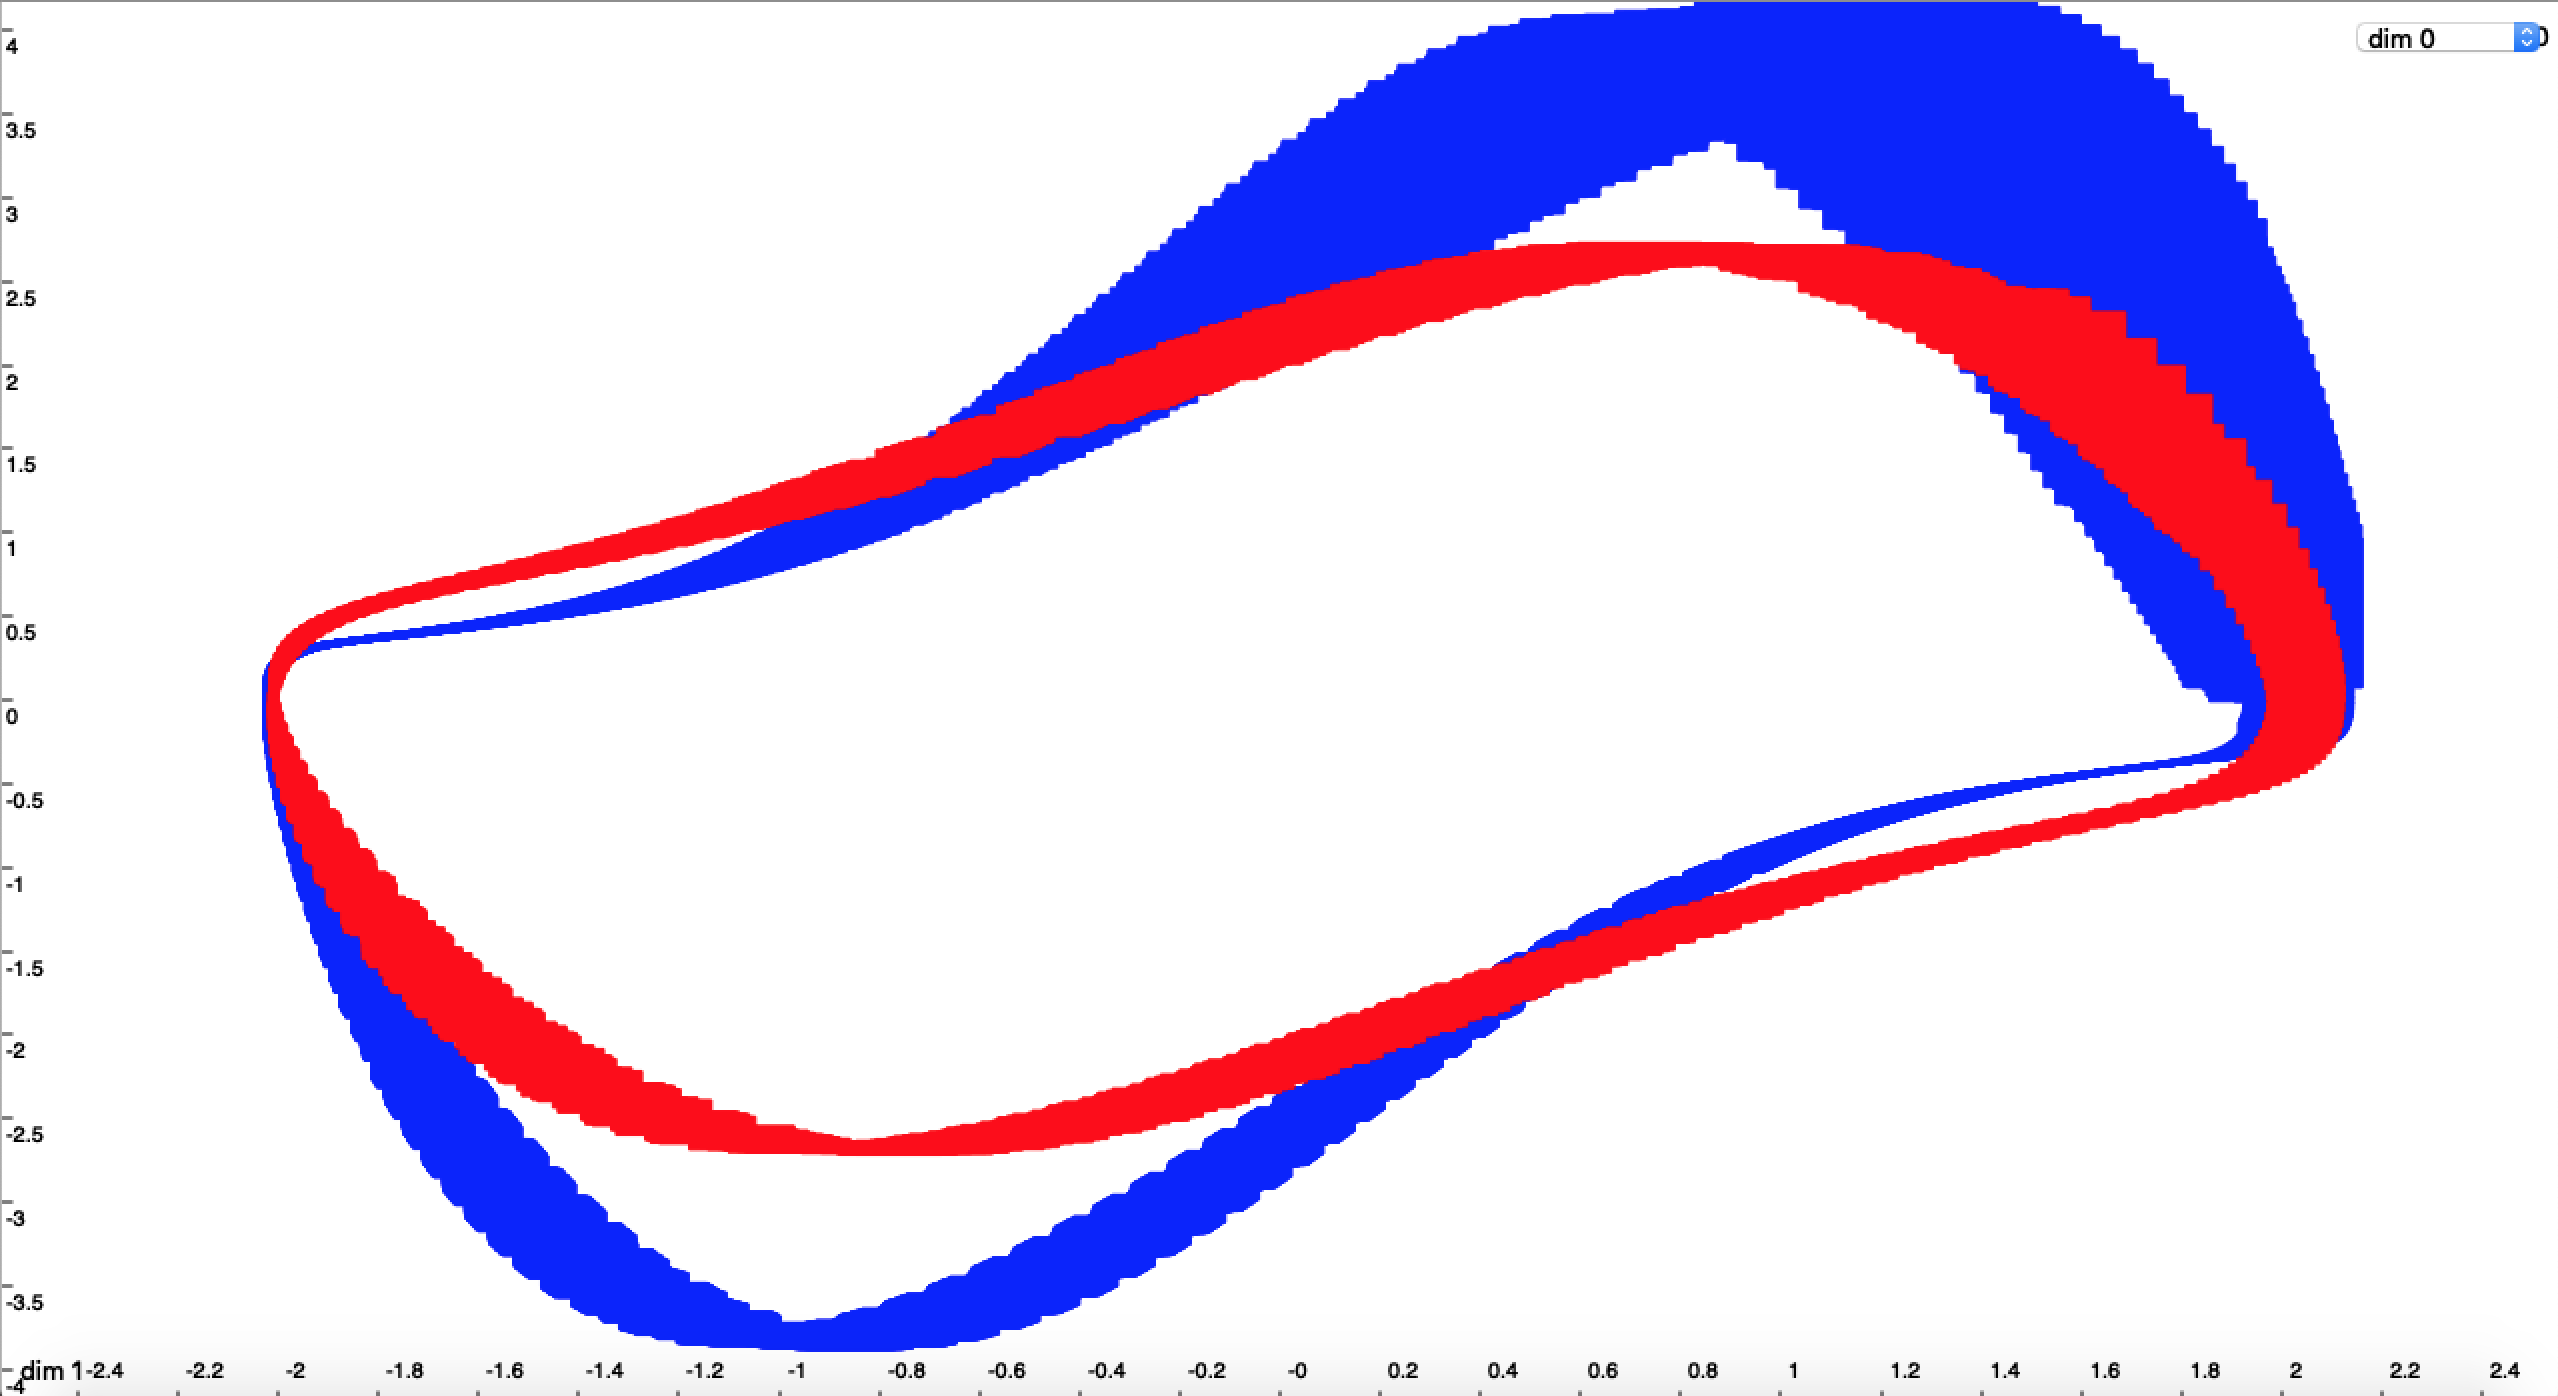
\includegraphics[width=5.5cm,height=5.5cm]{results_DynIbex/vdp.png}
  \label{fig:vanderpol:DynIbex}}
% %  \hspace{0.2in}
% \subfigure[CORA/SX.] 
% 	  {\includegraphics[width=5.5cm, height=5.5cm, trim=50 50 50 50, clip=true]{results_SpaceEx/.png}
%   \label{fig:vanderpol:CORASX}}
% %  \hspace{0.2in}
% \subfigure[C2E2.] 
% 	  {\includegraphics[width=5.5cm, height=5.5cm]{results_C2E2/.png}
%   \label{fig:vanderpol:C2E2}}
% %  \hspace{0.2in}
 \subfigure[Flow* ($\mu = 2$.] 
 	  {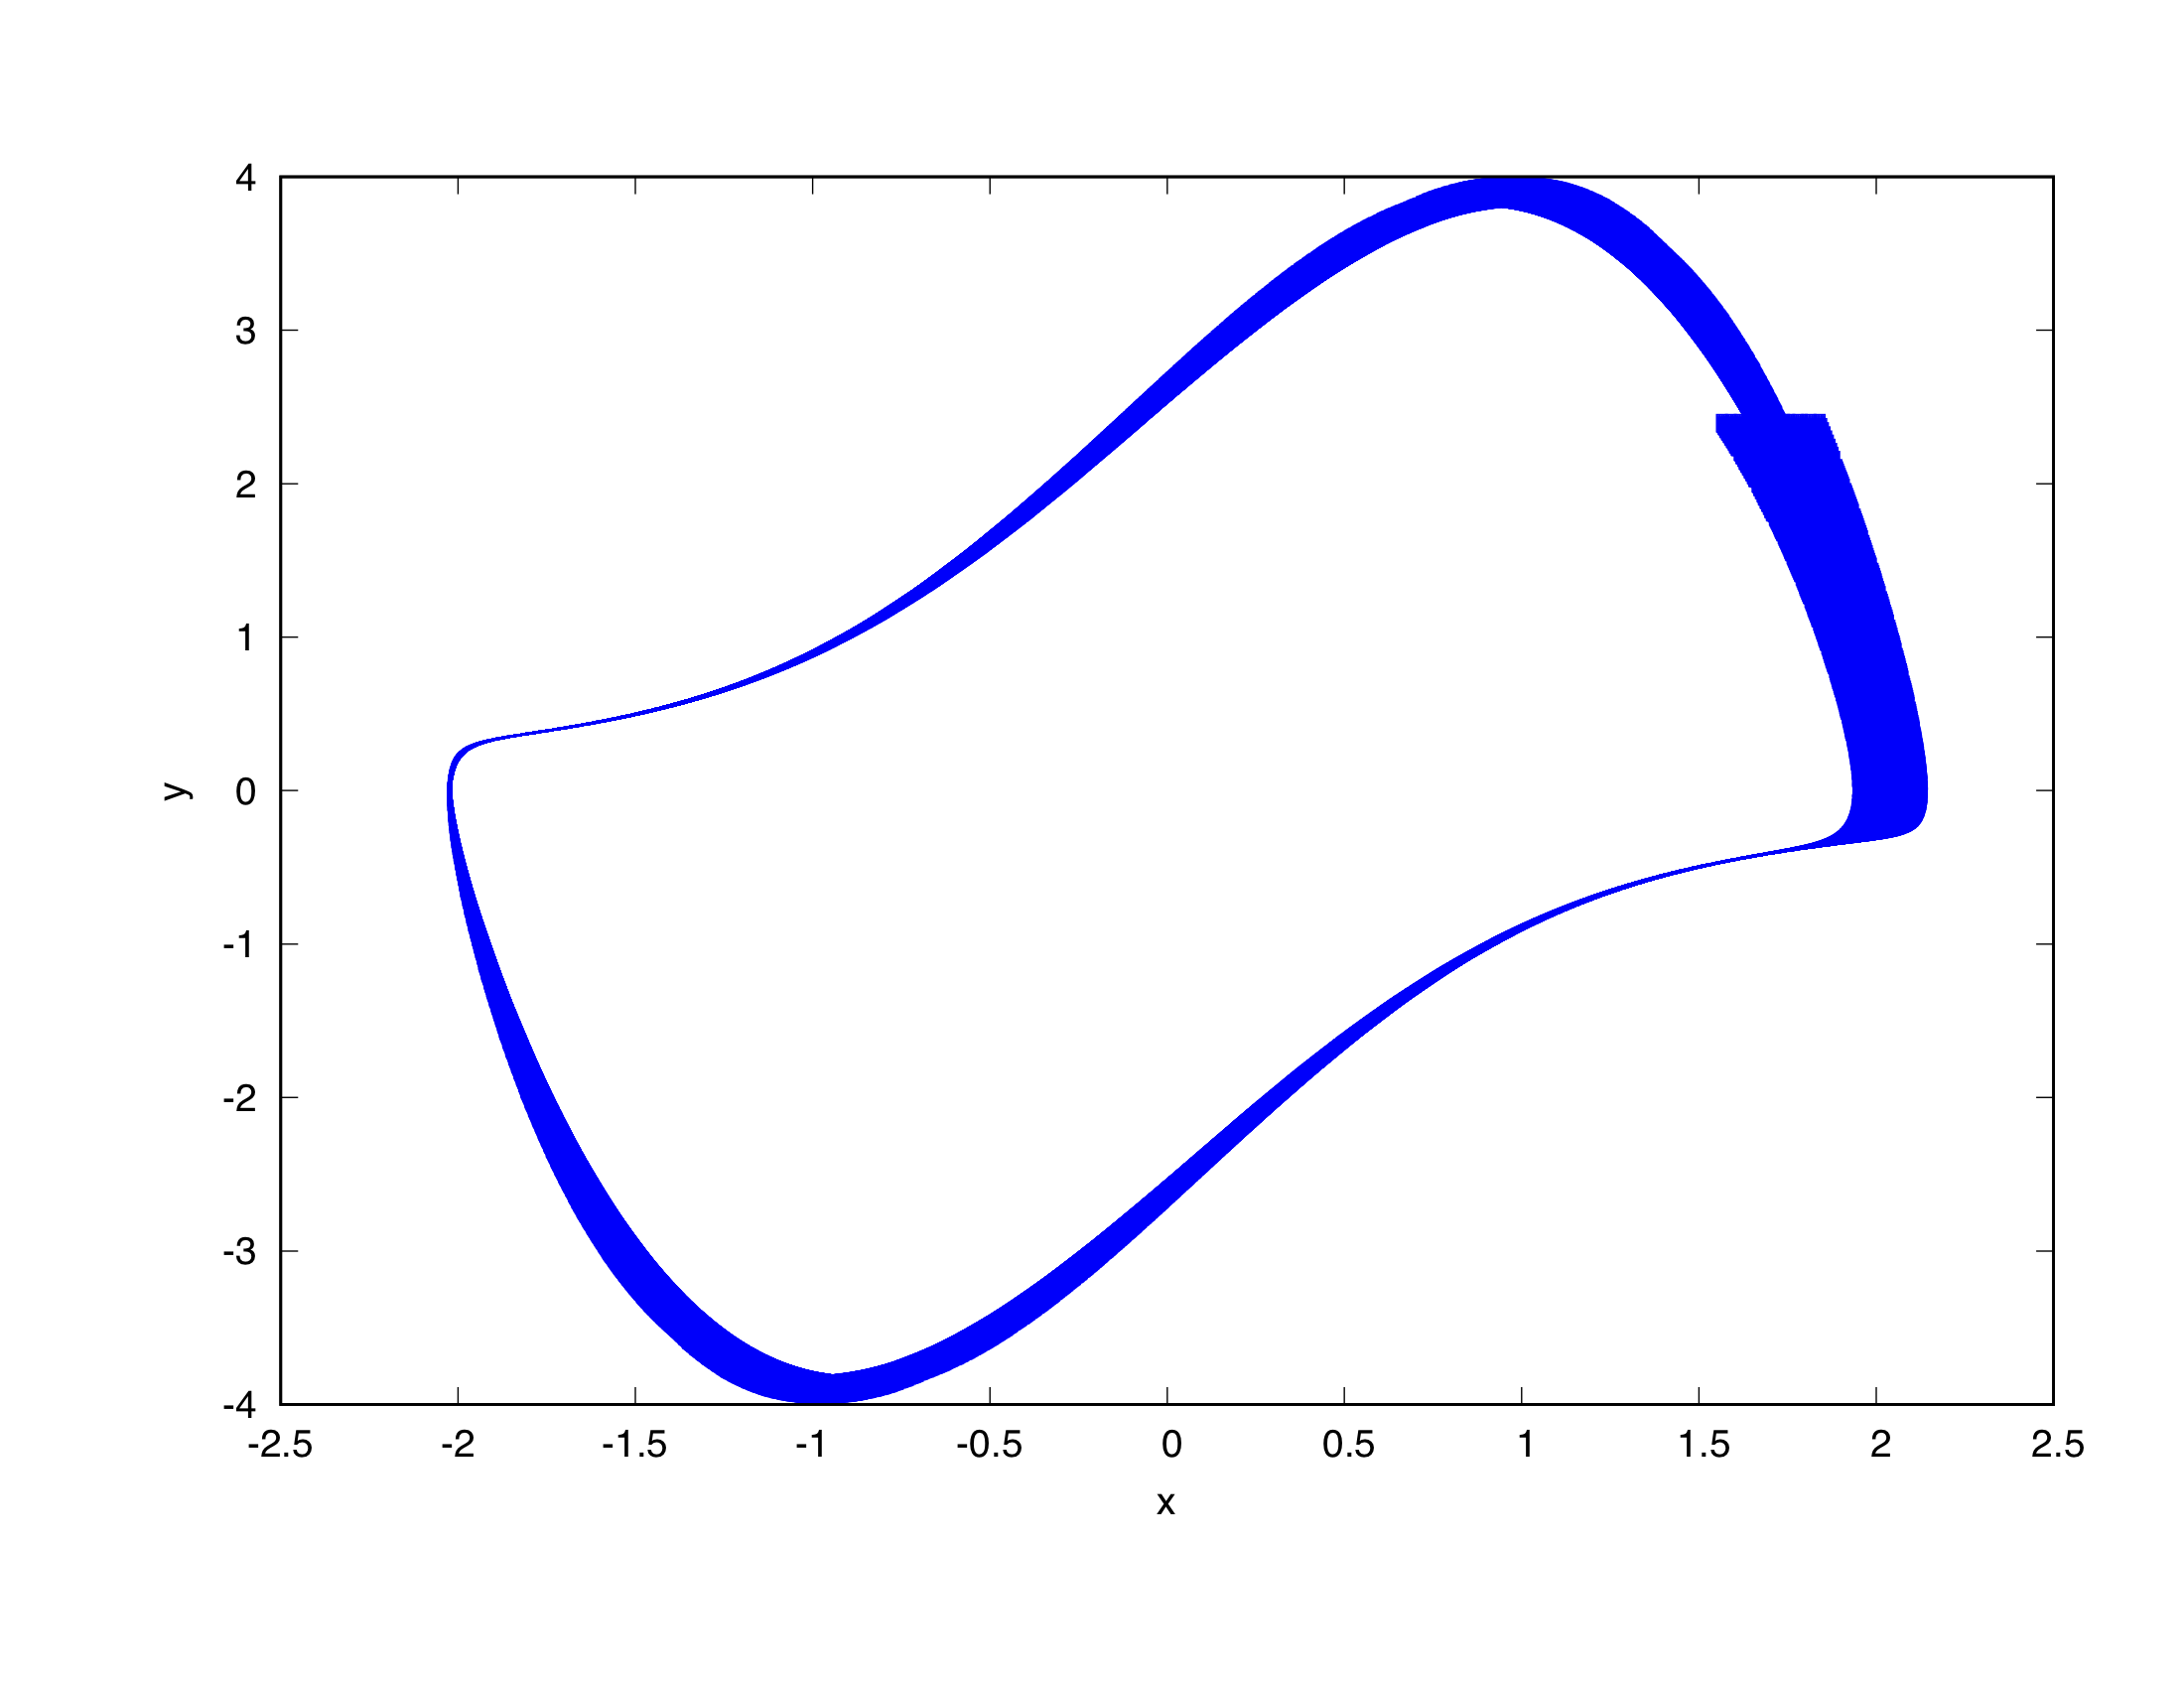
\includegraphics[width=5.5cm, height=5.5cm]{results_flowstar/vanderpol_2.png}
   \label{fig:vanderpol:flowstar}}
  \hspace{0.2in}
\subfigure[Isabelle/HOL.] 
	  {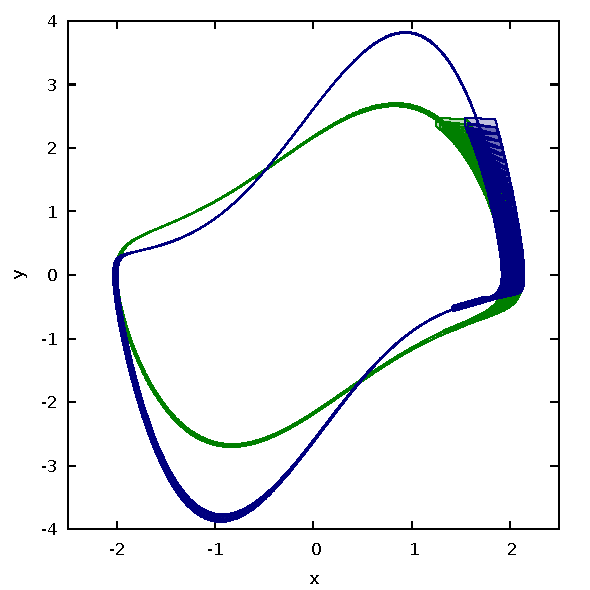
\includegraphics[width=5.5cm, height=5.5cm]{results_Isabelle/out_vdp.pdf}
  \label{fig:vanderpol:isabelle}}
%   \hspace{0.2in}
\subfigure[JuliaReach.] 
	  {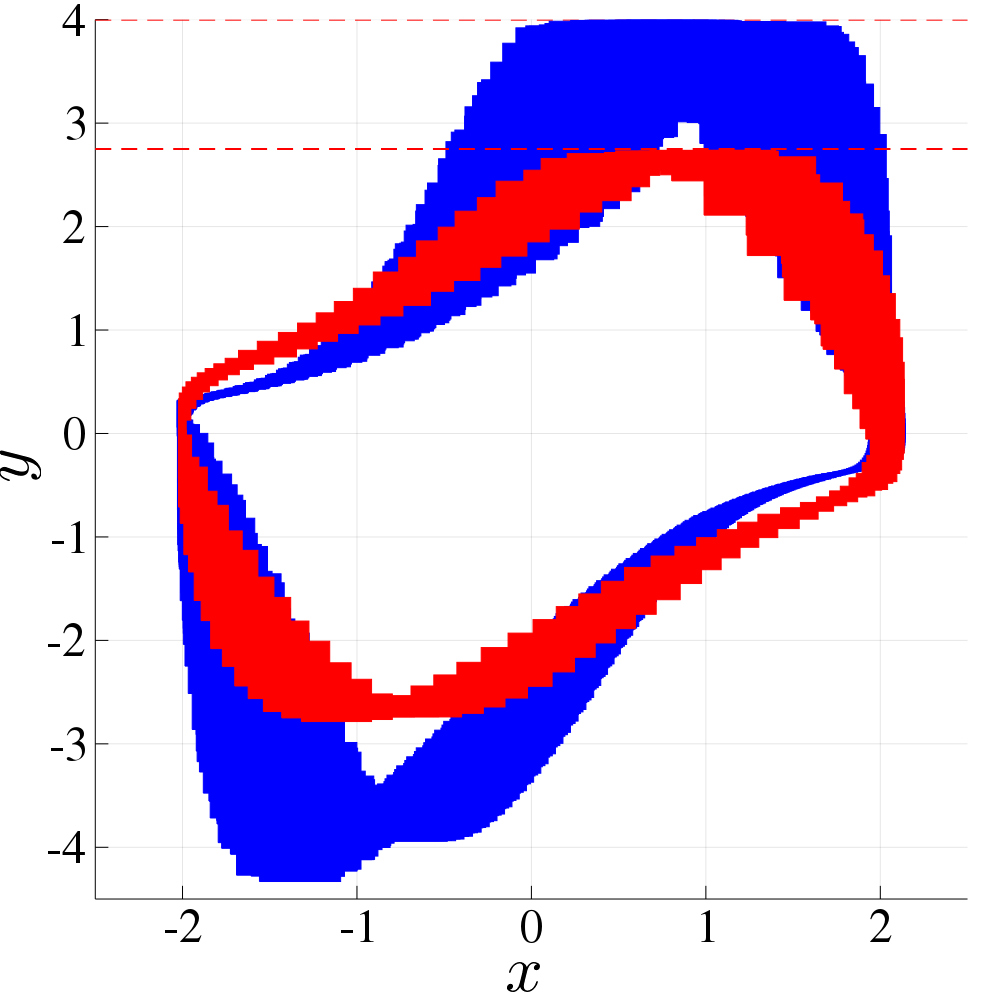
\includegraphics[width=5.5cm, height=5.5cm]{results_JuliaReach/vanderpol_case_all.png}
  \label{fig:vanderpol:Juliareach}}
\caption{Reachable set overapproximations for the Van der Pol oscillator. $x \in [-2.5, 2.5]$, $y \in [-4, 4]$.}
\label{fig:vanderpol}
\end{figure}

\begin{table}[t]
	\setlength{\tabcolsep}{4pt}
	\renewcommand{\arraystretch}{1.2}
	\centering
	\caption{Results of the Van der Pol Oscillator. Details of the platforms are described in Section~\ref{sec:machines}.}\label{tab:compTimes:vanderpol}
	\begin{tabular}[c]{lcccc}
	\hline
		   & \multicolumn{2}{c}{\textbf{computation time in [s]}} &  \multicolumn{2}{c}{\textbf{platform}} \\
        \cmidrule(l){2-3}
		 \textbf{tool} & \textbf{$\mu=1$} & \textbf{$\mu = 2$} & $\textbf{language}$ & $\textbf{machine}$ \\		 
		 \hline
		 Ariadne & $2.5$ & $33$ & C++ & M$_{\text{Ariadne}}$ \\
         CORA & $2.3$ & $2.8$ & MATLAB & M$_{\text{CORA}}$ \\
%         CORA/SX & $0.6$ & & C++ & M$_{\text{SpaceEx}}$ \\
         DynIbex & $16$ & $653$ & C++ &  M$_{\text{DynIbex}}$\\
         Flow* & $0.4$ & $8.7$ & C++ & M$_{\text{Flow*}}$ \\
         Isabelle/HOL & $1.4$ & $2.0$ & SML & M$_{\text{Isabelle}}$ \\
         JuliaReach & $0.7$ & $5.9$ & Julia & M$_{\text{JuliaReach}}$ \\
		 \hline
	\end{tabular}
\end{table}

\paragraph{Setting for Ariadne.}
For $\mu=1$, the maximum step size used is $0.02$, with a maximum temporal order of $5$. The maximum spacial error enforced for each step is $2 \cdot 10^{-4}$. For $\mu=2$, the maximum step size used is $0.04$, a maximum temporal order of $5$ and a maximum spacial error enforced for each step equal to $2 \cdot 10^{-4}$; in this case we also split the initial set into $16$ subsets by enforcing a maximum enclosure radius of $0.3$. While for $\mu=2$ the plotting (in dark gray) appears to cross the $y=4$ boundary, in fact it is overapproximated graphically and the reachable sets are proved to respect $y\leq3.96$.

\paragraph{Setting for CORA.}
For $\mu = 1$, a pseudo invariant at $x=1.5$ was introduced manually. For $\mu = 2$, two pseudo invariants at $x=1.8$ and $x=-1.8$ were introduced manually. CORA uses the time step size $0.01$ and the zonotope order $20$ for both cases $\mu = 1$ and $\mu = 2$.

% \paragraph{Setting for CORA/SX.}
% A pseudo invariant at $x=1.2$ was introduced manually. The time step size is $0.01$ and the zonotope order is chosen as $20$. 

% \paragraph{Setting for C2E2.} C2E2 proved the safety of the model by using time step size $0.01$. The K value is chosen to be 1000. The reachtube for variable $x$ is over bloated due to the lack of constraints on variable $x$. The reachtube overapproximation is enough for proving the safety constraints on variable $y$. Note that the result for C2E2 is not optimal since C2E2 is currently been updated.

\paragraph{Setting for DynIbex.}
Maximum zonotope order is set to $20$, reachability analysis is carried out with an (absolute and relative) error tolerance of $10^{-7}$ using an implicit midpoint Runge-Kutta method of order $2$. For $\mu=1$ a partition of the initial state in $16$ sub-boxes is performed. For $\mu=2$ a partition of the initial state in $256$ sub-boxes has been considered.

\paragraph{Setting for Flow*.}
For the model with $\mu = 1$, Flow* uses the following setting: a fixed stepsize of $0.04$, an adaptive order from $4$ to $8$, the cutoff threshold is set to be $10^{-6}$, the remainder estimation is $10^{-5}$ in all dimensions, the remainder queue size is $100$, and the precision is $100$. All roundoff errors are included in the TM flowpipes. The test case for $\mu = 2$ is more challenging, we used a fixed order of $6$ along with an adaptive stepsize from $0.001$ to $0.04$, the cutoff threshold is $10^{-8}$, and we increase the remainder queue size to $1000$. In order to prove the flowpipes are in the range of $y < 4$, we equally divide the initial set in the dimension of $x$ to $6$ pieces. Since Flow* does not provide the function to overlap grid plots, we show the flowpipes in the second test in Figure~\ref{fig:vanderpol:flowstar}.

%Flow* uses the step size $0.04$, the TM order $6$, the cutoff threshold $10^{-6}$, and the precision $53$ for floating-point numbers. The TM flowpipe remainders are kept symbolically every $100$ steps. All floating-point roundoff errors are included in the overapproximations. Since there are only $2$ state variables, the tool plots a grid overapproximation for the flowpipes, see Figure~\ref{fig:vanderpol:flowstar}. The approximation quality can be better evaluated based on the remainder size of the last TM flowpipe (see~\cite{Chen/2015/phd}). In this task, the overapproximation error for the last flowpipe is bounded by only $0.01214$.


\paragraph{Setting for Isabelle/HOL.}
Maximum Zonotope order is set to $20$, Reachability analysis is carried out with an (absolute and relative) error tolerance of $2^{-14}$. For $\mu = 1$ and $\mu = 2$, a pseudo-invariant is added at $x=1.5$. The case $\mu = 2$ is more demanding, it requires an additional pseudo-invariant  at $x = -1.5, y >= 0$.

\paragraph{Setting for JuliaReach.} For $\mu=1$, we used $n_Q=2$, $n_T=10$, and an absolute tolerance of $10^{-10}$, which leads to an average step size $\sim 0.06$. For $\mu=2$, in order to stay in the safe region, we split the set of initial states along the $x$-direction and used $n_Q=1$, $n_T=10$, and an absolute tolerance of $10^{-10}$.

\subsection{Laub-Loomis Benchmark}

\subsubsection{Model}

The Laub-Loomis model is presented in~\cite{Laub+Loomis/1998/oscillator} for studying a class of enzymatic activities. The dynamics can be defined by the following ODE with $7$ variables.
\[
\left\{
\begin{array}{lcl}
 \dot{x}_1 & = & 1.4 x_3 - 0.9 x_1 \\
 \dot{x}_2 & = & 2.5 x_5 - 1.5 x_2 \\
 \dot{x}_3 & = & 0.6 x_7 - 0.8 x_2 x_3 \\
 \dot{x}_4 & = & 2 - 1.3 x_3 x_4 \\
 \dot{x}_5 & = & 0.7 x_1 - x_4 x_5 \\
 \dot{x}_6 & = & 0.3 x_1 - 3.1 x_6 \\
 \dot{x}_7 & = & 1.8 x_6 - 1.5 x_2 x_7
\end{array}
\right.
\]
The system is asymptotically stable and the equilibrium is the origin.


\subsubsection{Specification}

The initial sets are defined according to the one used in~\cite{Testylier+/2013/NLTOOLBOX}. They are boxes centered at $x_1(0) = 1.2$, $x_2(0) = 1.05$, $x_3(0) =
1.5$, $x_4(0) = 2.4$, $x_5(0) = 1$, $x_6(0) = 0.1$, $x_7(0) = 0.45$. The range of the box in the $i$th dimension is defined by the interval $[x_i(0)-W, x_i(0)+W]$. The width $W$ of the initial set is vital to the difficulty of the reachability analysis job. The larger the initial set the harder the reachability analysis. 

We consider $W = 0.01$, $W = 0.05$, and $W = 0.1$.
For $W=0.01$ and $W=0.05$ we consider the unsafe region defined by $x_4 \geq 4.5$, while for $W=0.1$, the unsafe set is defined by $x_4 \geq 5$. The time horizon for all cases is $[0,20]$.


\subsubsection{Results}

The computation results of the tools are given in Table~\ref{tab:compTimes:laubloomis}. It can be seen that enlarging the initial set size can greatly make the reachability analysis task harder. The tool settings are given as below. Since the safety condition is only related to the variable $x_4$, we present the plots of projections of the overapproximations in the $t$-$x_4$ plane such that $t$ is the time variable. Figure~\ref{fig:laubloomis:1} shows the results.
%for the smaller initial set ($W = 0.01$), Figure~\ref{fig:laubloomis:2} for the larger one ($W = 0.1$). 

\begin{table}[t]
	\setlength{\tabcolsep}{4pt}
	\renewcommand{\arraystretch}{1.2}
	\centering
	\caption{Results of the Laub-Loomis model. Details of the platforms are described in Section~\ref{sec:machines}.}
	\begin{tabular}[c]{lccccc}
	\hline
		 & \multicolumn{3}{c}{\textbf{computation time in [s]}} & \multicolumn{2}{c}{\textbf{platform}} \\ \cmidrule(l){2-4} \cmidrule(l){5-6}
		 \textbf{tool} & \textbf{$W=0.01$} & \textbf{$W=0.05$} & \textbf{$W=0.1$} & $\textbf{language}$ & $\textbf{machine}$ \\ \hline
		 Ariadne & $7.7$ & $1039$ & $1317$ & C++ & M$_{\text{Ariadne}}$ \\
         CORA & $0.82$ & $18$ & $56$ & MATLAB & M$_{\text{CORA}}$ \\
%         CORA/SX & $0.85$ & & -- & C++ & M$_{\text{SpaceEx}}$ \\
         DynIbex & $20$ & $64$ & $-$ & C++ & M$_{\text{DynIbex}}$ \\
         Flow* & $1.1$ & $2.8$ & $4.9$ & C++ & M$_{\text{Flow*}}$ \\
         Isabelle/HOL & $11$ & $18$ & $-$ & SML & M$_{\text{Isabelle}}$ \\
         JuliaReach & $3.4$ & $3.3$ & $3.4$ & Julia & M$_{\text{JuliaReach}}$ \\
		 \hline
	\end{tabular} \\[1em]
	\begin{tabular}[c]{lccc}
	\hline
		 & \multicolumn{3}{c}{\textbf{width of $x_4$ in final enclosure}}\\
		 \cmidrule(l){2-4}
		 \textbf{tool} & \textbf{$W=0.01$} & \textbf{$W=0.05$} & \textbf{$W=0.1$} \\ \hline
		 Ariadne & $0.05$ & $0.10$ & $1.96$ \\
         CORA & $0.02$ & $0.07$ & $0.11$\\
%         CORA/SX & & & \\
         DynIbex & $0.103$ & $ 0.403$ & $-$\\
         Flow* & $0.0049$ & $0.0253$ & $0.0444$ \\
         Isabelle/HOL & $0.06$ & $0.45$ & $\infty$ \\
         JuliaReach & $0.01$ & $0.03$ & $0.05$ \\
		 \hline
	\end{tabular}
	\label{tab:compTimes:laubloomis}
\end{table}


\begin{figure}[p]
\centering
\subfigure[Ariadne] 
	  {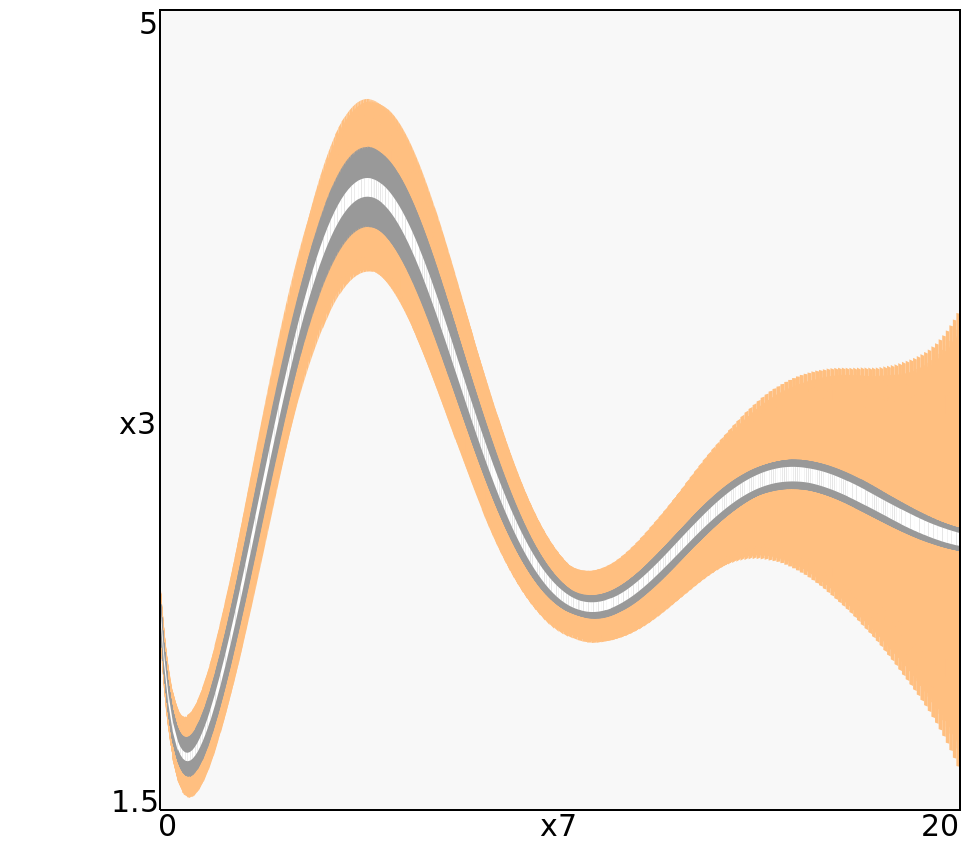
\includegraphics[width=5.5cm, height=5.0cm]{results_Ariadne/laubloomis.png}
  \label{fig:laubloomis:ariadne}}
  \hspace{0.2in}
\subfigure[CORA] 
	  {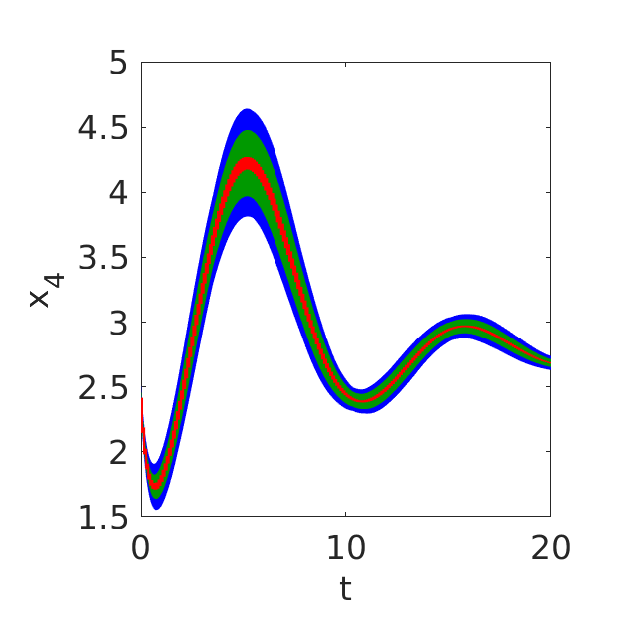
\includegraphics[width=5.5cm, height=5.5cm]{results_CORA/laubLoomis_27March2019.eps}
  \label{fig:laubloomis:cora:smaller}}
  \hspace{0.2in}
% \subfigure[CORA/SX] 
% 	  {\includegraphics[width=5.5cm, height=5.5cm,trim=50 50 50 50,clip=true]{results_SpaceEx/.png}
%   \label{fig:laubloomis:corasx:smaller}}\\
% \subfigure[C2E2] 
% 	  {\includegraphics[width=5.5cm, height=5.5cm]{results_C2E2/.png}
%   \label{fig:laubloomis:C2E2:smaller}}
%   \hspace{0.2in}
 \subfigure[DynIbex] 
 	  {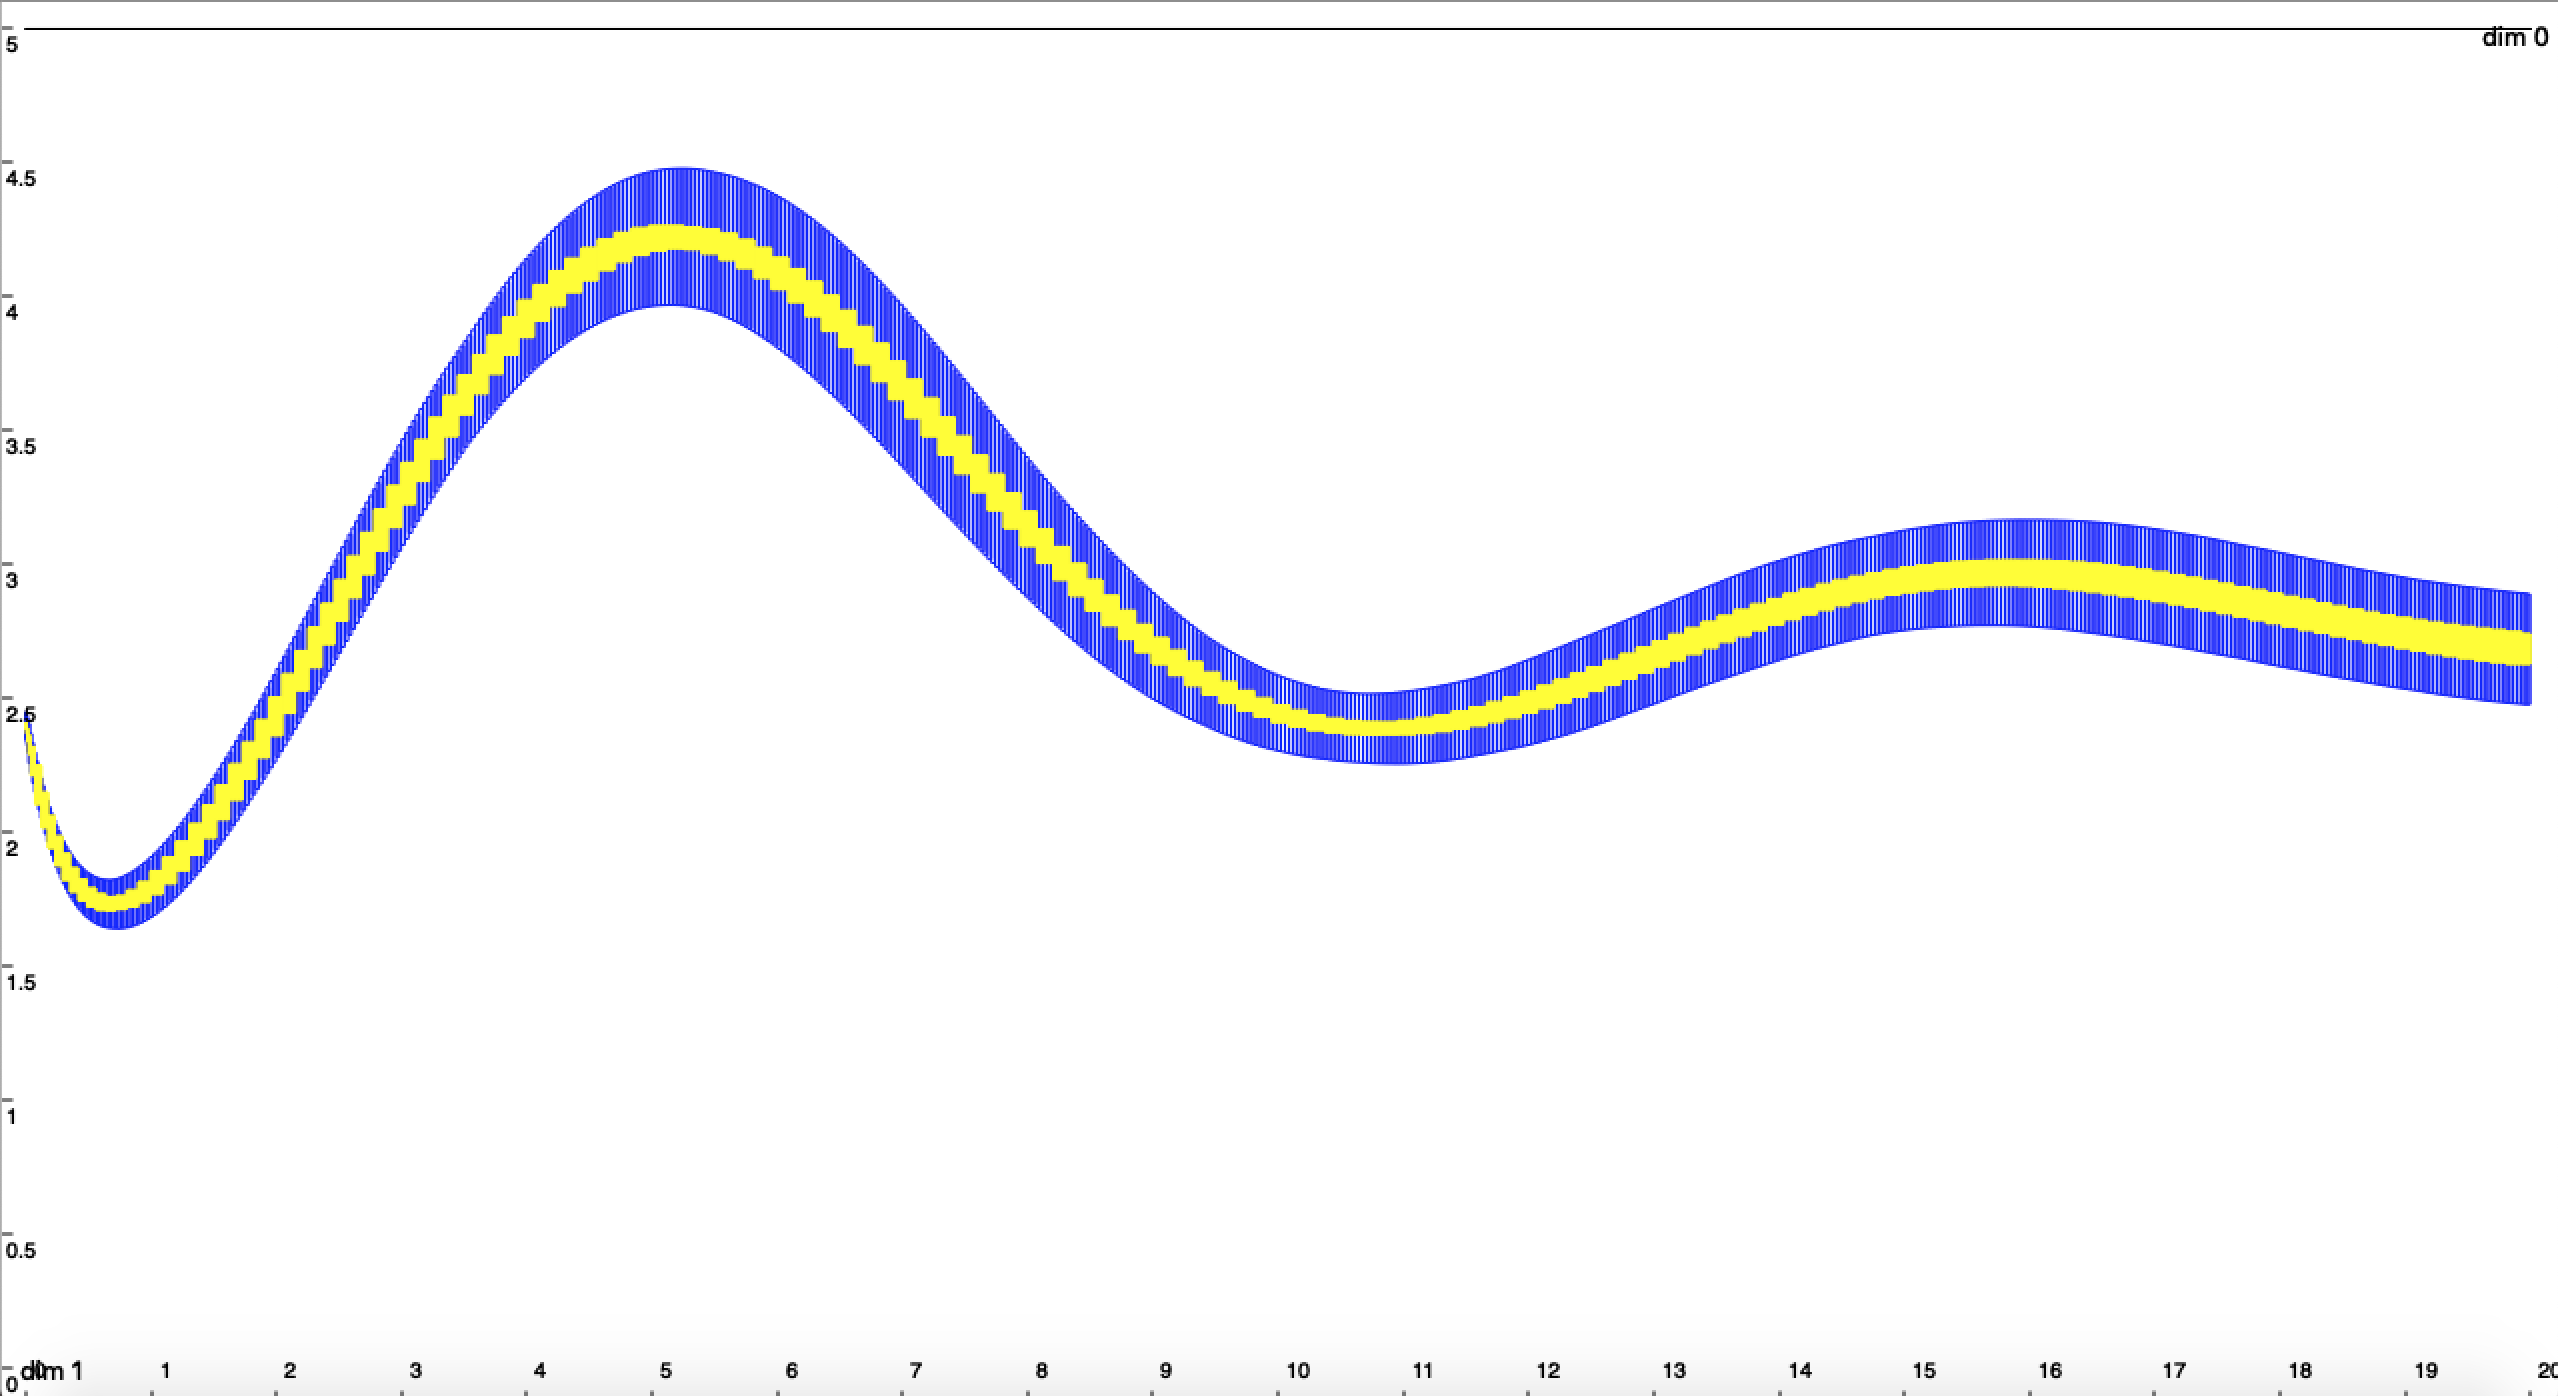
\includegraphics[width=5.5cm, height=5.5cm]{results_DynIbex/laub-loomis.png}
 \label{fig:laubloomis:DynIbex:smaller}}
 \subfigure[Flow*] 
 	  {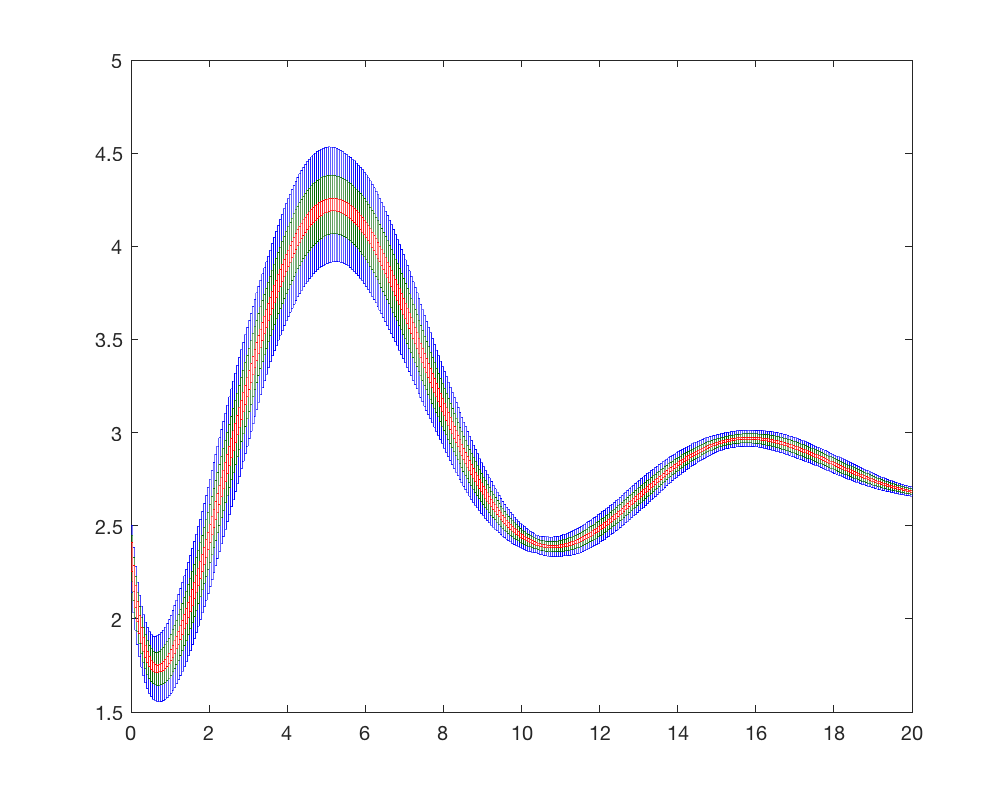
\includegraphics[width=5.5cm, height=5.5cm]{results_flowstar/laub_loomis.png}
   \label{fig:laubloomis:flowstar}}
   \hspace{0.2in}
\subfigure[Isabelle/HOL] 
	  {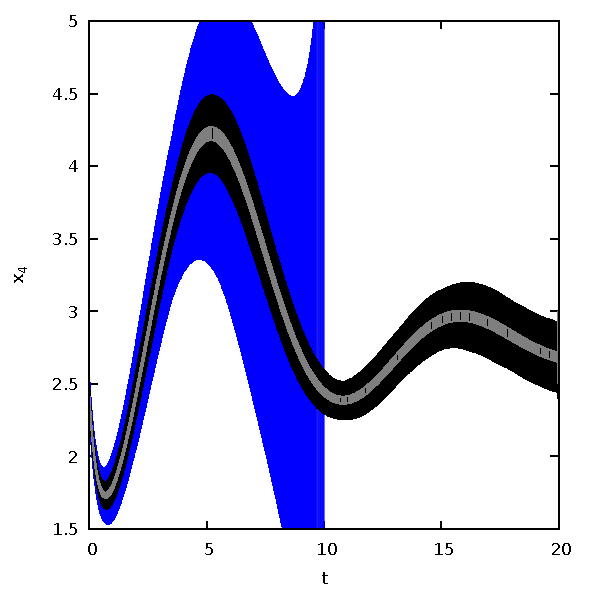
\includegraphics[width=5.5cm, height=5.5cm]{results_Isabelle/out_ll.pdf}
  \label{fig:laubloomis:isabelle}}
\hspace{0.2in}
\subfigure[JuliaReach.] 
	  {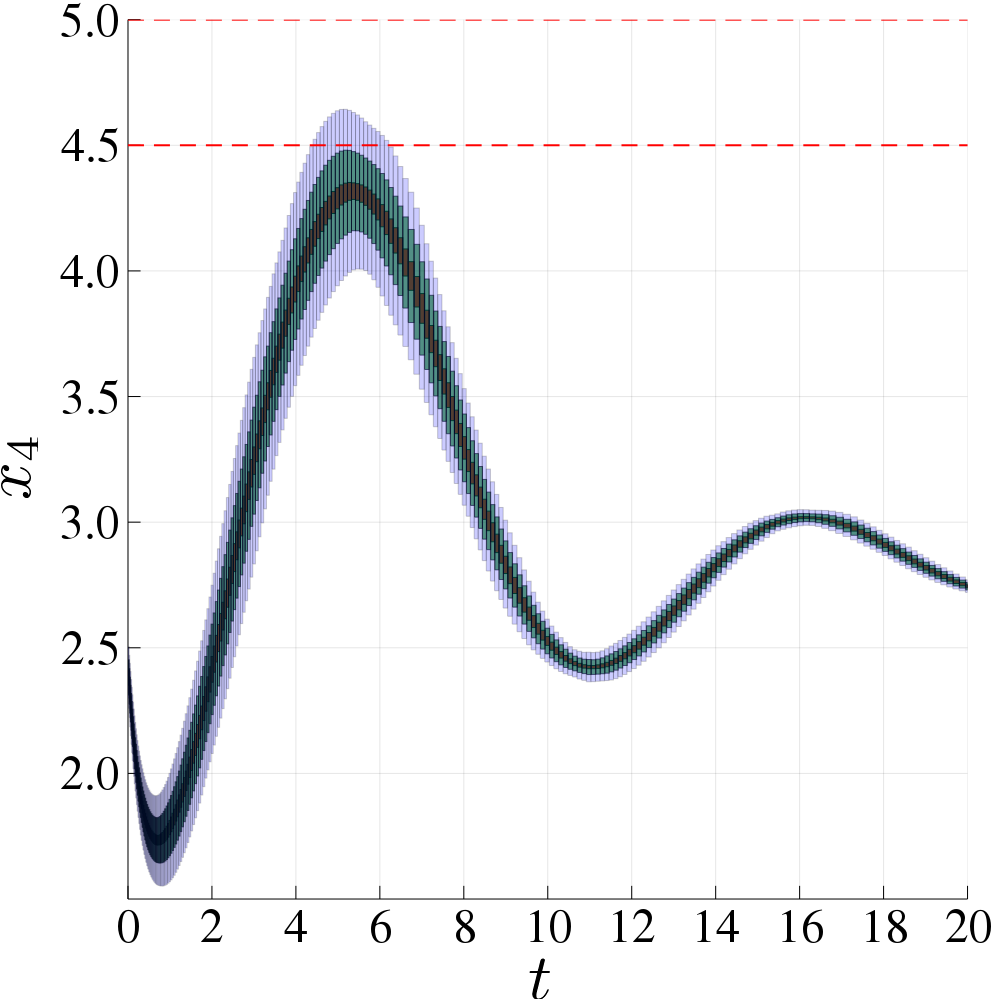
\includegraphics[width=5.5cm, height=5.5cm]{results_JuliaReach/laubloomis_case_all.png}
  \label{fig:laubloomis:JuliaReach}}
\hspace{0.2in}
\caption{Reachable set overapproximations for the Laub-Loomis model (Overlayed plots for $W = 0.01$,
$W = 0.05$, $W = 0.1$). $t \in [0, 20]$, $x_4 \in [1.5, 5]$.}
\label{fig:laubloomis:1}
\end{figure}

%  \begin{figure}[t]
%  \centering
% \subfigure[CORA] 
% 	  {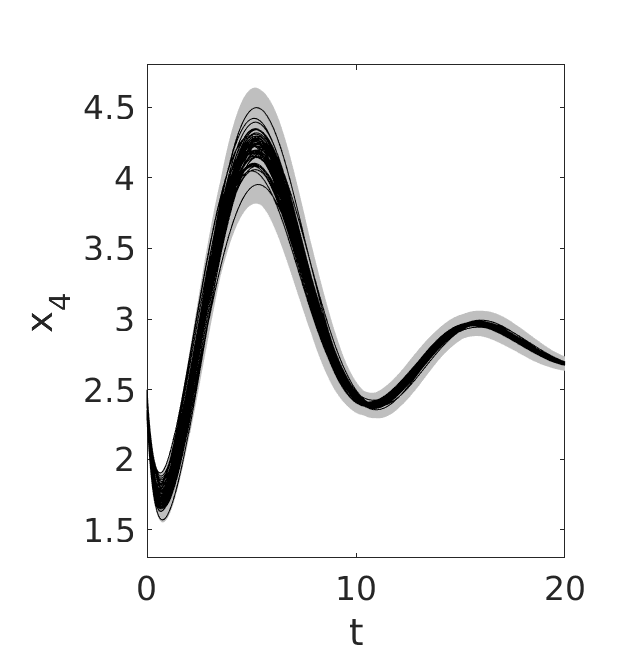
\includegraphics[width=5.5cm, height=5.5cm]{results_CORA/laubLoomis_W01_30May2018.eps}
%   \label{fig:laubloomis:cora:larger}}
% \subfigure[C2E2] 
% 	  {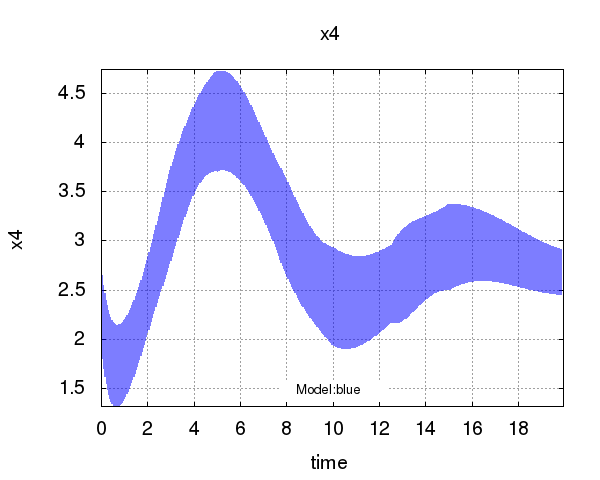
\includegraphics[width=5.5cm, height=5.5cm]{results_C2E2/laub_large.png}
%   \label{fig:laubloomis:C2E2:larger}}
%     \hspace{0.2in}
% \subfigure[Flow*] 
% 	  {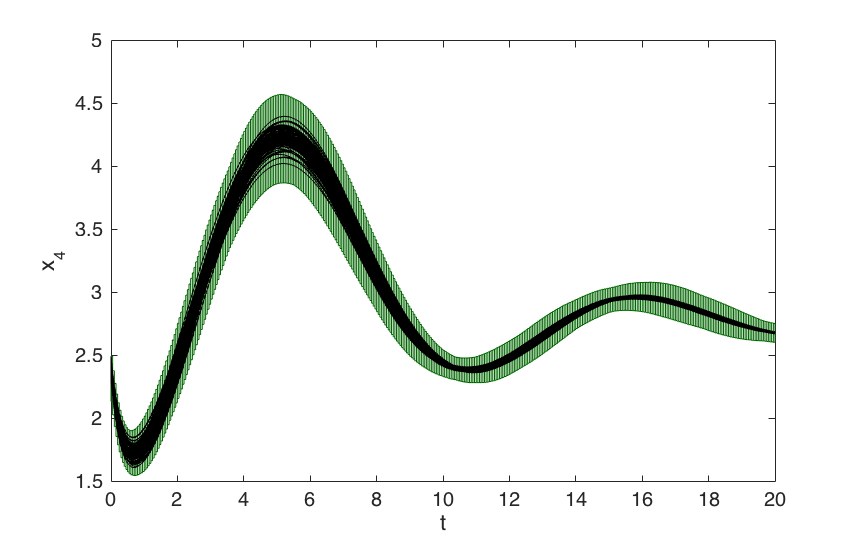
\includegraphics[width=5.5cm, height=5.5cm]{results_flowstar/laub_loomis_large.png}
%   \label{fig:laubloomis:flowstar:larger}}
% %\hspace{0.24in}
% %\subfigure[SymReach: $W = 0.1$] 
% %	  {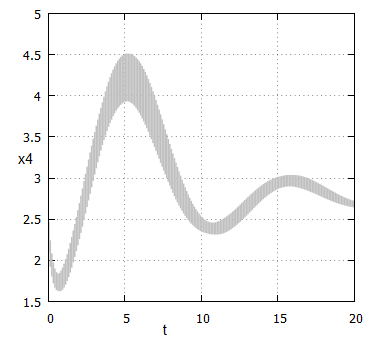
\includegraphics[width=0.45\columnwidth, height=5cm]{results_SymReach/laubloomisW0p1.png}
% %  \label{fig:laubloomis:SymReach:larger}}
%  \caption{Reachable set overapproximations for the Laub-Loomis model ($W = 0.1$).}
%  \label{fig:laubloomis:2}
%  \end{figure}

\clearpage

\paragraph{Setting for Ariadne.}
The maximum step size used is $0.2$, the temporal order is $4$ and a maximum spacial error enforced for each step equal to $2 \cdot 10^{-3}$. For $W=0.05$ and $W=0.1$ a splitting strategy for the initial set is used; the strategy compares the radius of the set with a reference value, respectively $0.03$ and $0.09$, in order to split once for each dimension and yield a total of $128$ initial subsets (the minimum amount using the current splitting strategy).

\paragraph{Setting for CORA.}
Depending on the size of the initial set, different algorithms in CORA are applied. For the smaller initial sets $W = 0.01$ and $W = 0.05$, the faster but less accurate algorithm presented in \cite{Althoff2008c} is executed. For the larger initial set $W = 0.1$, the more accurate but slower algorithm from \cite{Althoff2013a} is used. CORA uses a step size of $0.1$ for $W = 0.01$, a step size of $0.025$ for $W = 0.05$, and a step size of $0.01$ for $W = 0.1$. The maximum zonotope order for all initial sets is chosen as $50$.

% \paragraph{Setting for CORA/SX.}
% Since CORA/SX does not currently support splitting the initial states, only the small initial set was handled. The time step is $0.1$ and the zonotope order is $50$.

\paragraph{Setting for DynIbex.}
For $W=0.01$ the maximum zonotope order is set to $50$ and the reachability analysis is carried out with an (absolute and relative) error tolerance of $10^{-5}$ with an explicit Runge-Kutta method of order $3$. For $W=0.05$ the maximum zonotope order is set to $80$ and the reachability analysis is carried out with an (absolute and relative) error tolerance of $10^{-7}$ with an explicit Runge-Kutta method of order $3$. For $W=0.01$ and $W=0.05$ no splitting of the initial conditions is performed. %For $W=0.1$ the same settings as for $W=0.05$ is used except that the zonotope order is $110$ and a splitting of the initial states in $64$ sub-boxes is performed.

\paragraph{Setting for Flow*.}
For all of the $3$ tests, Flow* uses a fixed stepsize of $0.05$, an adaptive order from $3$ to $8$, and a cutoff threshold of $10^{-7}$. The remainder estimation is $10^{-4}$ in all dimensions and we set the precision to $100$ for floating-point numbers. For the initial set sizes $W = 0.01$ and $W = 0.05$, we set the remainder queue size to $100$, while for $W=0.1$, we raise the queue size to $200$. The new version of Flow* shows a much better performance than the previous one which is presented last year, however the accuracy is nearly the same or even better.

%For the small initial set, Flow* uses the step size $0.1$, the TM order $4$, the cutoff threshold $10^{-7}$ and the precision $53$ for floating-point numbers. The TM flowpipe remainders are kept symbolically every $50$ steps. Besides the safety set that is defined by $x_4 \leq 4.5$, the tool even proves that $x_4 \leq 4.3$ is safe. On the other hand, for the large initial set, we use the same setting except that the stepsize is reduced to $0.05$, and the remainders are kept symbolically every $100$ steps. Besides the given safety property, the tool proves a smaller safe set which is defined by $x_4 \leq 4.6$. The plots of the flowpipes are shown in Figure~\ref{fig:laubloomis:flowstar:smaller} and~\ref{fig:laubloomis:flowstar:larger}. Notice that they are only the interval overapproximations of the flowpipes, the exact flowpipes are much more accurate, since for the small initial set, the maximum overapproximation error of the last flowpipe is only $0.01044$ which is determined by the $x_4$-dimension, while for the large initial set, the corresponding maximum error is only $0.06016$.


\paragraph{Setting for Isabelle/HOL.}
Maximum Zonotope order is set to $60$. Reachability analysis is carried out with an (absolute and relative) error tolerance of $2^{-12}$. We do not perform subdivisions of the initial set. This results in failure to maintain precise enclosures for $W=0.1$ and $t \ge 7$


\paragraph{Setting for JuliaReach.} We used $n_Q=1$, $n_T=7$ and an absolute tolerance of $10^{-10}$ for the three cases.


\subsection{Quadrotor Benchmark}

\subsubsection{Model}

We study the dynamics of a quadrotor as derived in \cite[eq. (16) - (19)]{Beard2008}. Let us first introduce the variables required to describe the model: The inertial (north) position $x_1$, the inertial (east) position $x_2$, the altitude $x_3$, the longitudinal velocity $x_4$, the lateral velocity $x_5$, the vertical velocity $x_6$, the roll angle $x_7$, the pitch angle $x_8$, the yaw angle $x_9$, the roll rate $x_{10}$, the pitch rate $x_{11}$, and the yaw rate $x_{12}$. We further require the following parameters: gravity constant $g = 9.81$ [m/s$^2$], radius of center mass $R = 0.1$ [m], distance of motors to center mass $l = 0.5$ [m], motor mass $M_{rotor} = 0.1$ [kg], center mass $M = 1$ [kg], and total mass $m = M + 4M_{rotor}$.

From the above parameters we can compute the moments of inertia as 
\begin{equation*}
\begin{split}
J_x =& \frac{2}{5} \, M \, R^2 + 2 \, l^2 \, M_{rotor}, \\
J_y =& J_x, \\
J_z =& \frac{2}{5} \, M \, R^2 + 4 \, l^2 \, M_{rotor}.
\end{split}
\end{equation*}

Finally, we can write the set of ordinary differential equations for the quadrotor according to \cite[eq. (16) - (19)]{Beard2008}:
\[
\left\{
\begin{array}{lcl}
\dot{x}_1 & = & \cos(x_8)\cos(x_9)x_4 + \Big(\sin(x_7)\sin(x_8)\cos(x_9) - \cos(x_7)\sin(x_9)\Big)x_5 \\
& & + \Big(\cos(x_7)\sin(x_8)\cos(x_9) + \sin(x_7)\sin(x_9)\Big)x_6 \\
\dot{x}_2 & = & \cos(x_8)\sin(x_9)x_4 + \Big(\sin(x_7)\sin(x_8)\sin(x_9) + \cos(x_7)\cos(x_9)\Big)x_5 \\
& & + \Big(\cos(x_7)\sin(x_8)\sin(x_9) - \sin(x_7)\cos(x_9)\Big)x_6 \\
\dot{x}_3 & = & \sin(x_8)x_4 - \sin(x_7)\cos(x_8)x_5 - \cos(x_7)\cos(x_8)x_6 \\
\dot{x}_4 & = & x_{12}x_5 - x_{11}x_6 - g\sin(x_8) \\
\dot{x}_5 & = & x_{10}x_6 - x_{12}x_4 + g\cos(x_8)\sin(x_7) \\
\dot{x}_6 & = & x_{11}x_4 - x_{10}x_5 + g\cos(x_8)\cos(x_7) - \frac{F}{m} \\
\dot{x}_7 & = & x_{10} + \sin(x_7)\tan(x_8)x_{11} + \cos(x_7)\tan(x_8)x_{12} \\
\dot{x}_8 & = & \cos(x_7)x_{11} - \sin(x_7)x_{12} \\
\dot{x}_9 & = & \frac{\sin(x_7)}{\cos(x_8)}x_{11} + \frac{\cos(x_7)}{\cos(x_8)}x_{12} \\
\dot{x}_{10} & = & \frac{J_y - J_z}{J_x}x_{11}x_{12} + \frac{1}{J_x}\tau_\phi \\
\dot{x}_{11} & = & \frac{J_z - J_x}{J_y}x_{10}x_{12} + \frac{1}{J_y}\tau_\theta \\
\dot{x}_{12} & = & \frac{J_x - J_y}{J_z}x_{10}x_{11} + \frac{1}{J_z}\tau_\psi 
\end{array}
\right.
\]

To check interesting control specifications, we stabilize the quadrotor using simple PD controllers for height, roll, and pitch. The inputs to the controller are the desired values for height, roll, and pitch $u_1$, $u_2$, and $u_3$, respectively. The equations of the controllers are
\[
\begin{array}{lcll}
F & = & m \, g - 10(x_3 - u_1) + 3x_6 \; & (\text{height control}), \\
\tau_\phi & = & -(x_7 - u_2) - x_{10} & (\text{roll control}), \\
\tau_\theta & = & -(x_8 - u_3) - x_{11} & (\text{pitch control}).
\end{array}
\]

We leave the heading uncontrolled so that we set $\tau_\psi = 0$.

\subsubsection{Specification}
The task is to change the height from $0$~[m] to $1$~[m] within $5$~[s]. A goal region $[0.98,1.02]$ of the height $x_3$ has to be reached within $5$~[s] and the height has to stay below $1.4$ for all times. After $1$~[s] the height should stay above $0.9$~[m]. The initial position of the quadrotor is uncertain in all directions within $[-0.4,0.4]$~[m] and also the velocity is uncertain within $[-0.4,0.4]$~[m/s] for all directions. All other values are initialized as $0$.

% The task is to move south-east for 2.5[s] and then stabilize height at 1 for 7.5[s]:
% \begin{itemize}
%     \item for t in [0, 2.5], set target (height,roll,pitch) to (1, 0.1, 0.25)
%     \item for t in [2.5, 10], set target (height,roll, pitch) to (1, 0, 0)
% \end{itemize} 
% At t=10[s], height must be in [0.98, 1.02], and the quadcopter shall be in the target area 
% of (north, east) in ([-60, -30], [10, 30]). The initial position of the quadrotor is uncertain in all directions within $[-0.4,0.4]$~[m] and also the velocity is uncertain within $[-0.4,0.4]$~[m/s] for all directions. All other values are initialized as $0$.

%\[
%\left\{
%\begin{array}{lcl}
% \dot{x} & = & \cos(\theta) \cos(\psi) p + (\sin(\phi) \sin(\theta) \cos(\psi) - \cos(\phi) \sin(\psi)) q + (\cos(\phi) \sin(\theta) \cos(\psi) + \sin(\phi) \sin(\psi)) r \\
% \dot{y} & = & \cos(\theta) \sin(\phi) p + (\sin(\phi) \sin(\theta) \sin(\psi) + \cos(\phi) \cos(\psi)) q + (\cos(\phi) \sin(\theta) \sin(\psi) - \sin(\phi) \cos(\psi)) r \\
% \dot{h} & = & \sin(\theta) p - \sin(\phi) \cos(\theta) q - \cos(\phi) \cos(\theta) r \\
% \dot{p} & = & w q - v r - 9.81 \sin(\theta) \\
% \dot{q} & = & u r - w p + 9.81 \cos(\theta \sin(\phi)) \\
% \dot{r} & = & v p - u q + 9.81 \cos(\theta \cos(\phi)) - 9.81 + 7.14285714285714 (h - 1) - 2.14285714285714 \, r \\
% \dot{\phi} & = & u + (\sin(\phi) \tan(\theta)) v + (\cos(\phi) \tan(\theta)) w \\
% \dot{\theta} & = & \cos(\phi) v - \sin(\phi) w \\
% \dot{\psi} & = & (\sin(\phi)/\cos(\theta)) v + (\cos(\phi)/\cos(\theta)) w \\
% \dot{u} & = & -0.92592592592593 v w - 18.51851851851852 (\phi + u) \\
% \dot{v} & = & 0.92592592592593 u w - 18.51851851851852 (\theta + v) \\
% \dot{w} & = & 0 \\
%\end{array}
%\right.
%\]

\begin{figure}[htb]
\centering
\subfigure[Ariadne.] 
	  {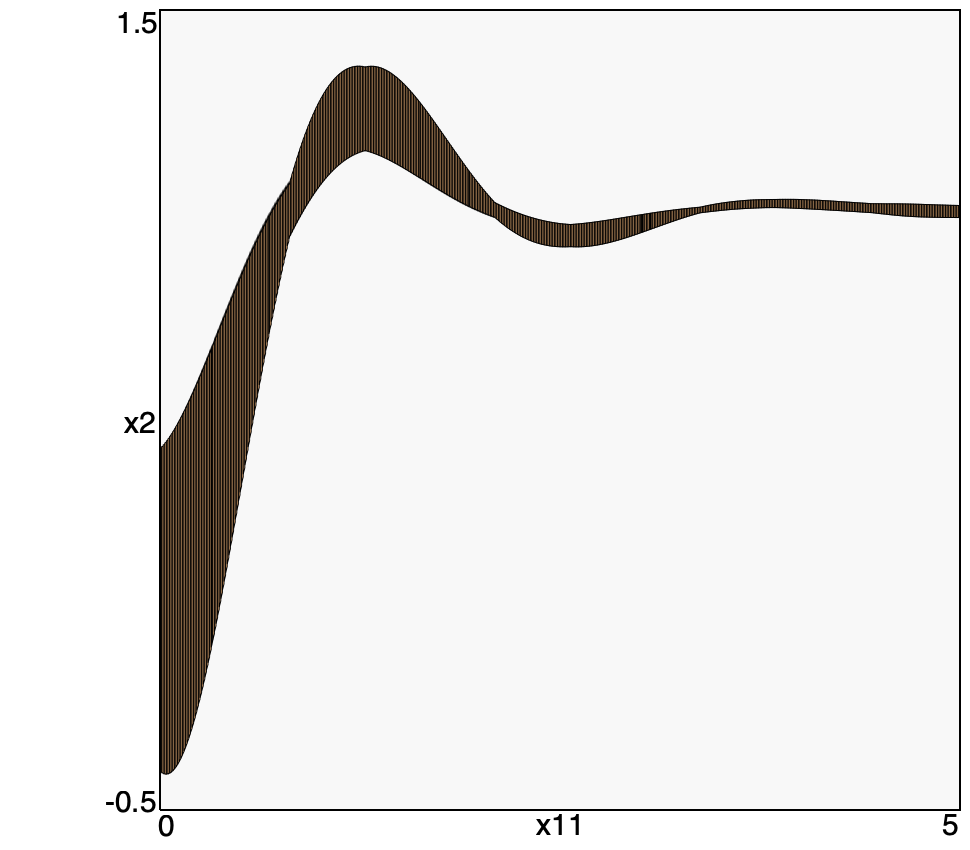
\includegraphics[width=5.5cm, height=5.0cm]{results_Ariadne/quadrotor.png}
  \label{fig:quadrotor:ariadne}}
  \hspace{0.2in}
\subfigure[CORA.] 
	  {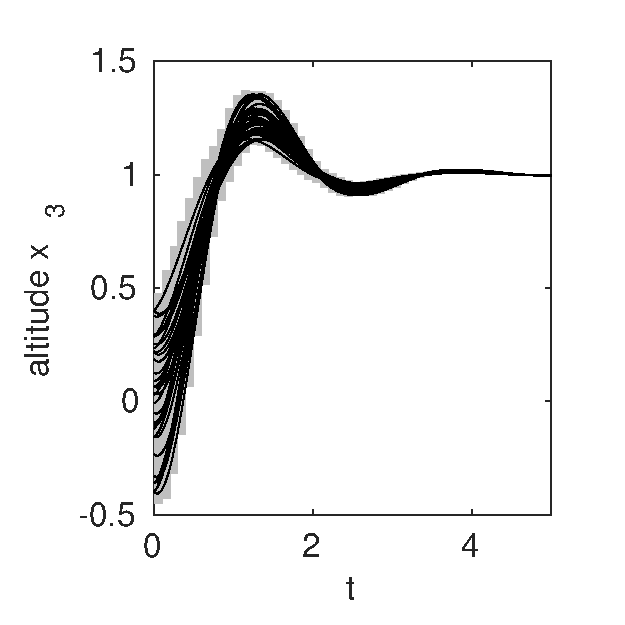
\includegraphics[width=5.5cm, height=5.5cm]{results_CORA/quadrotor_13March2019.eps}
  \label{fig:quadrotor:cora}}
  \hspace{0.2in}
% \subfigure[CORA/SX.] 
% 	  {\includegraphics[width=5.5cm, height=5.5cm,trim=50 50 50 75, clip=true]{results_SpaceEx/.png}
%   \label{fig:quadrotor:corasx}}
%   \hspace{0.2in}
  \subfigure[DynIbex.] 
	  {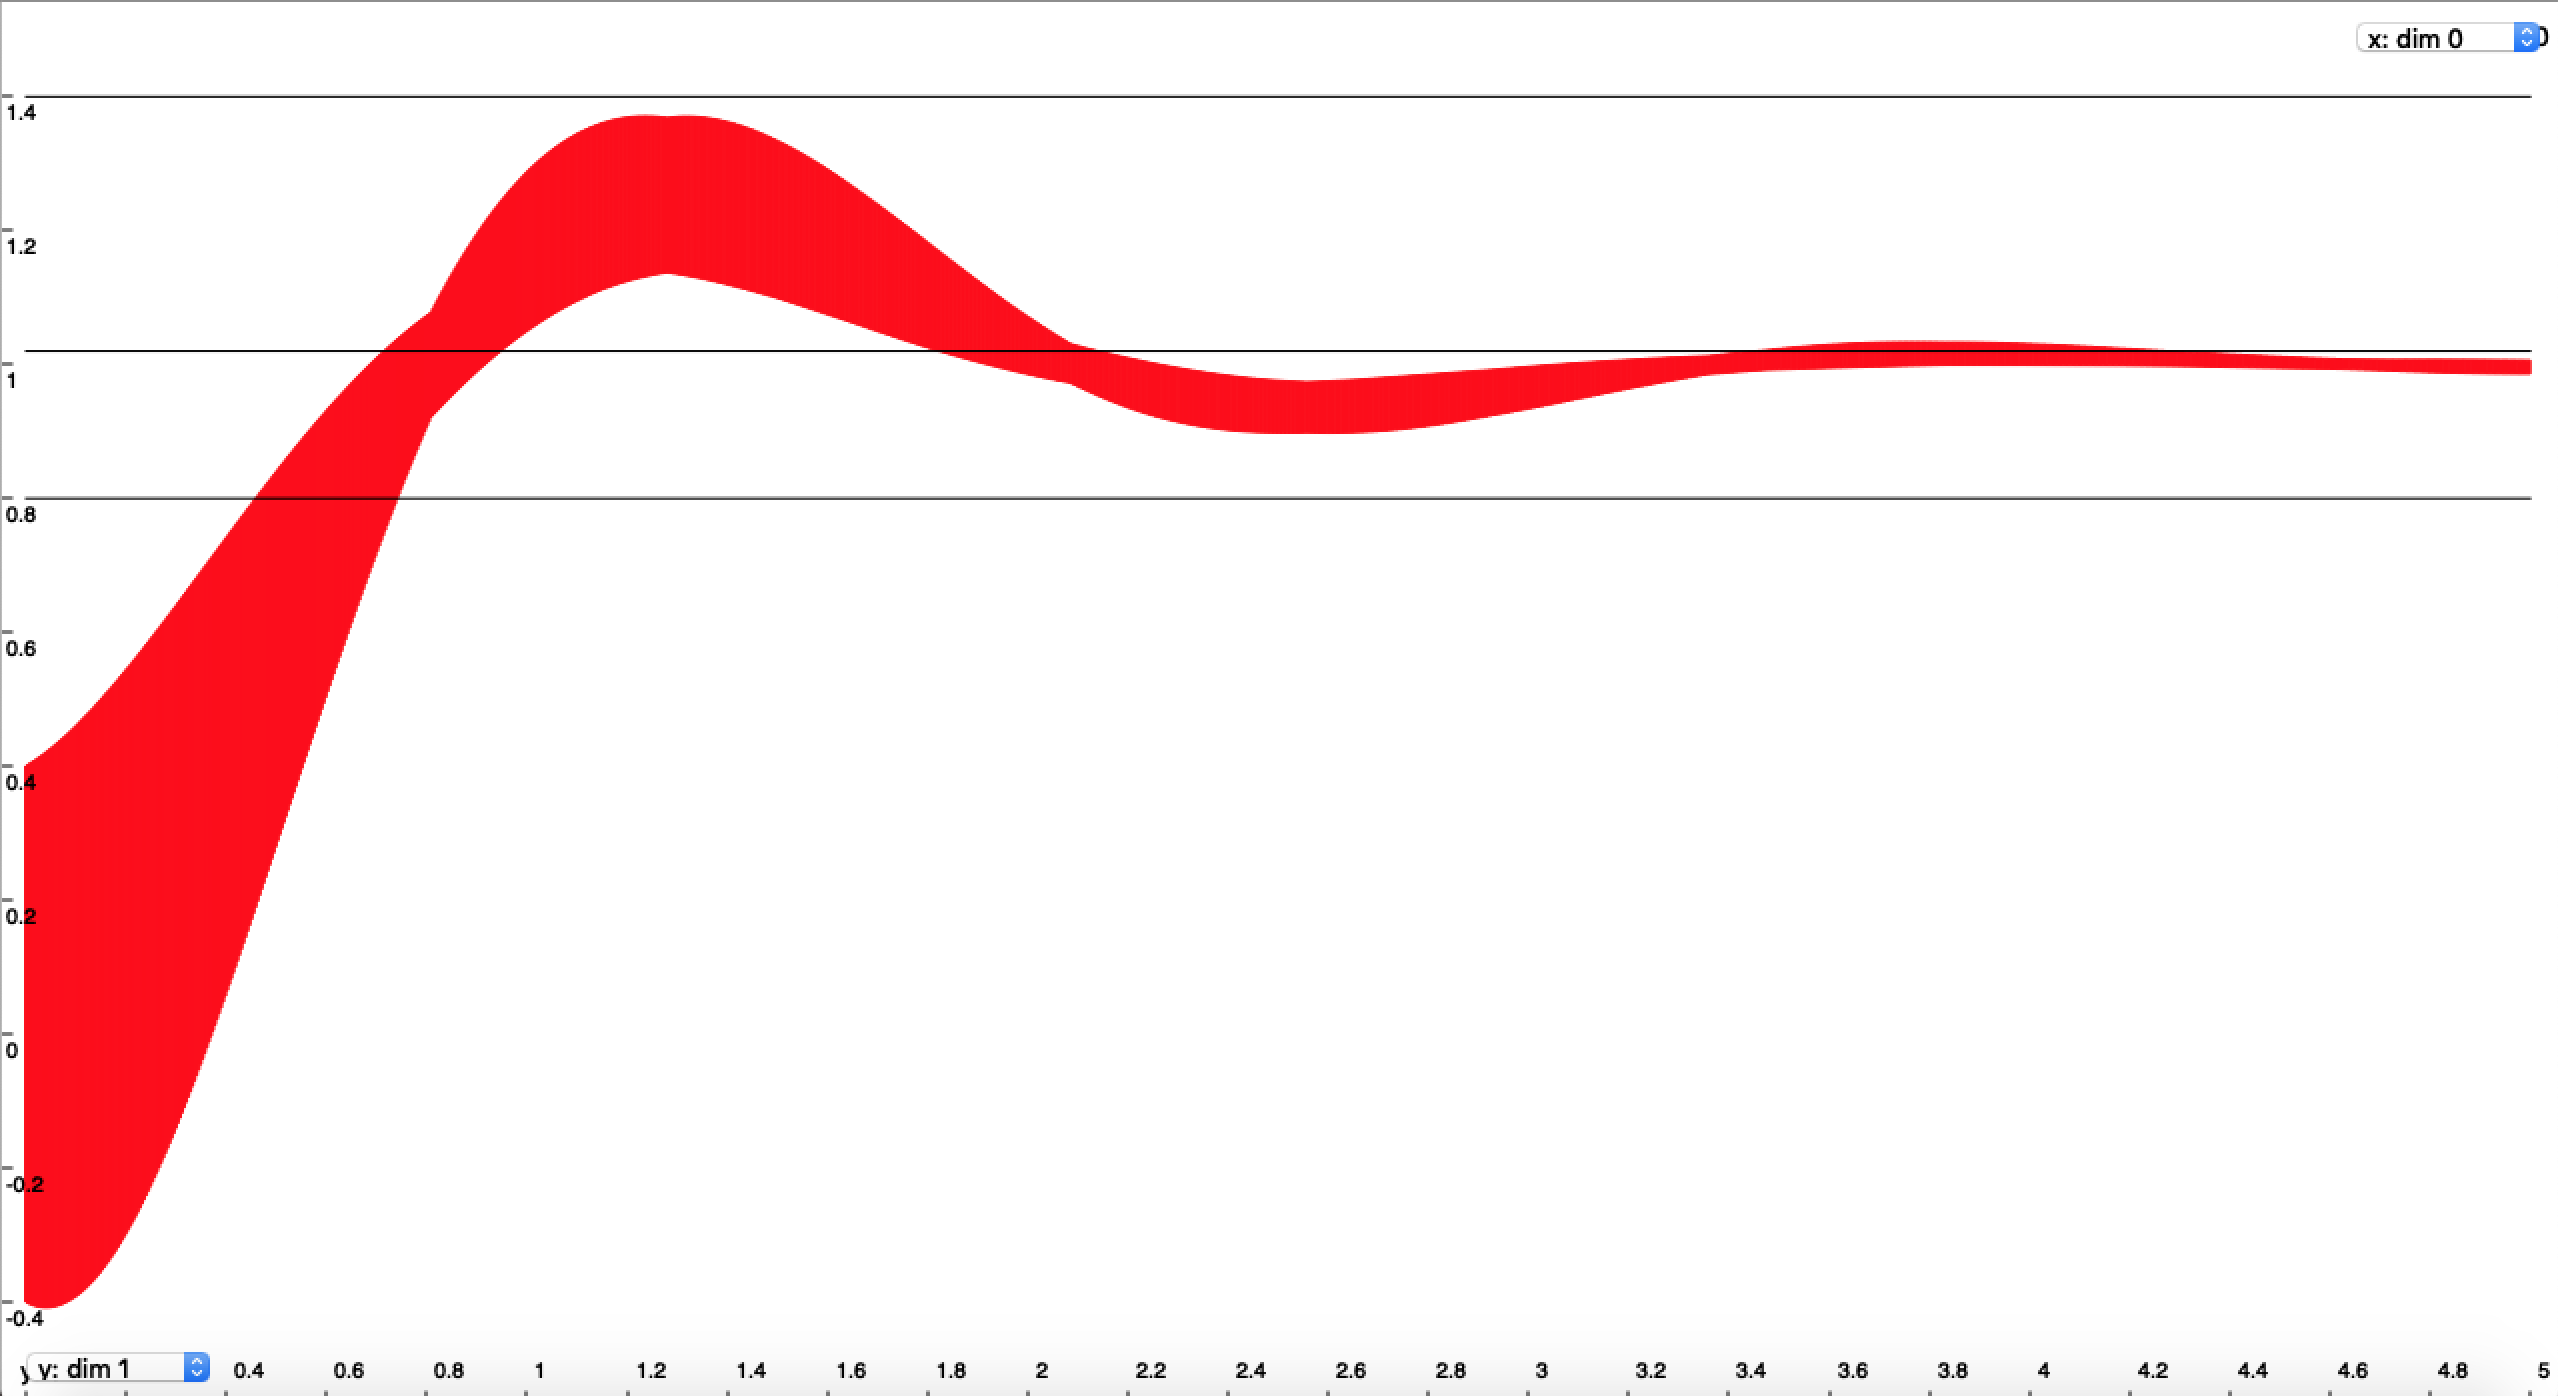
\includegraphics[width=5.5cm, height=5.5cm]{results_DynIbex/quadrotor.png}
  \label{fig:quadrotor:DynIbex}}
 \subfigure[Flow*.] 
 	  {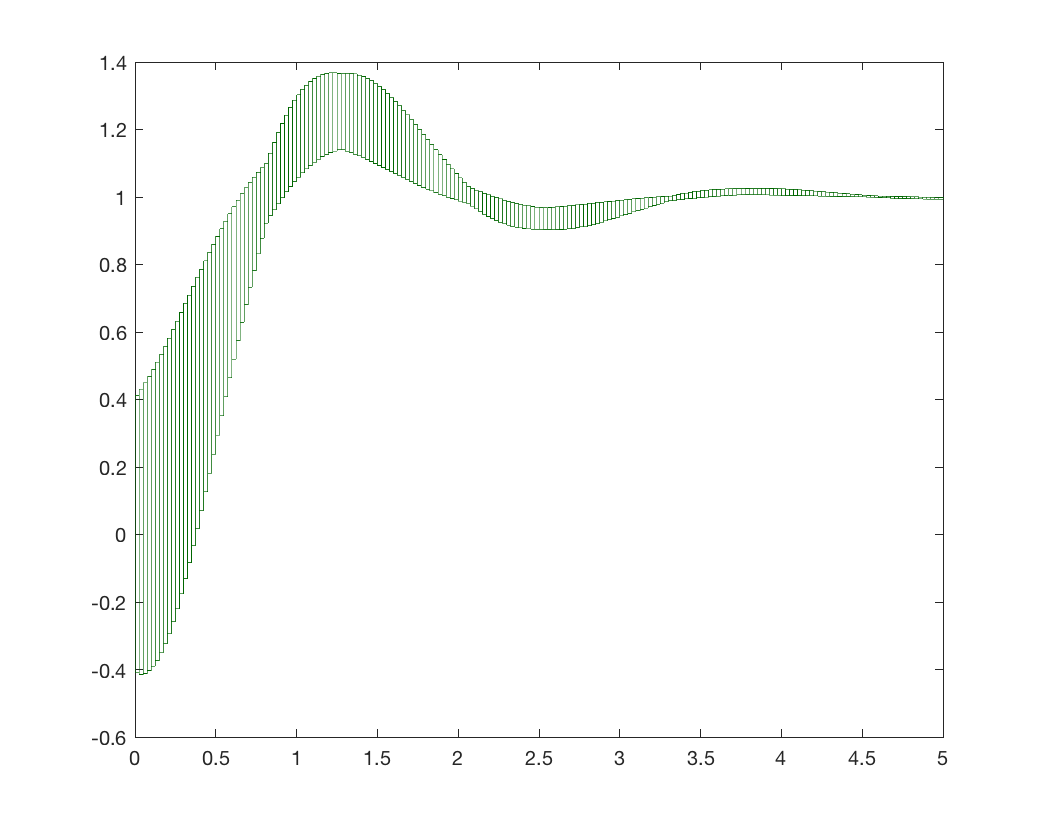
\includegraphics[width=5.5cm, height=5.5cm]{results_flowstar/Quadrotor.png}
   \label{fig:quadrotor:flow*}}
\subfigure[Isabelle/HOL.] 
	  {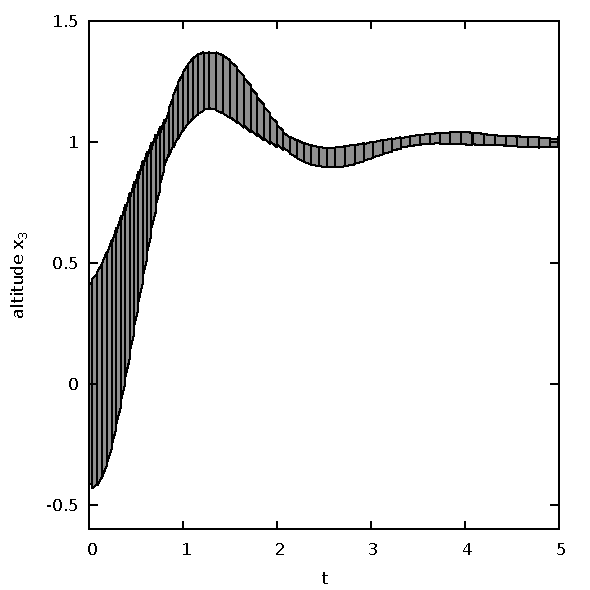
\includegraphics[width=5.5cm, height=5.5cm]{results_Isabelle/out_quadrot.pdf}
  \label{fig:quadrotor:isabelle}}
\subfigure[JuliaReach.] 
	  {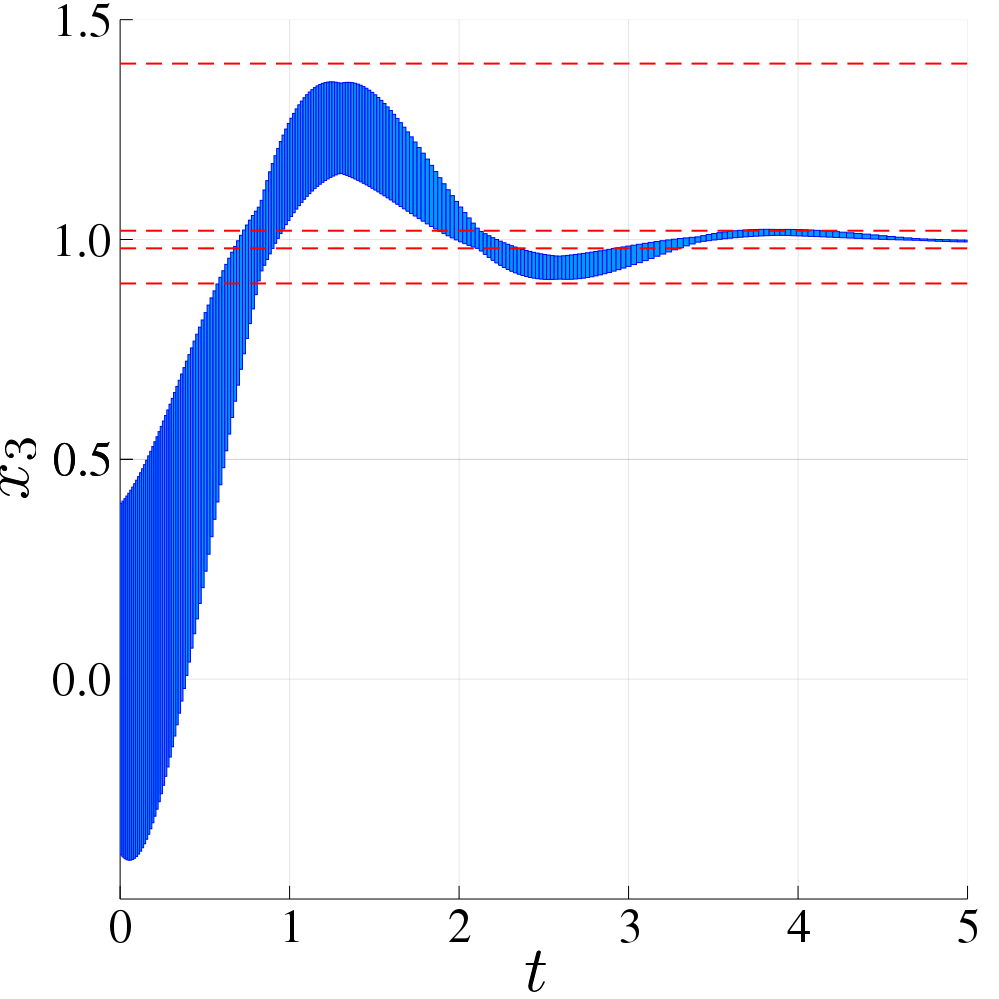
\includegraphics[width=5.5cm, height=5.5cm]{results_JuliaReach/quadrotor.png}
  \label{fig:quadrotor:JuliaReach}}
% \subfigure[SymReach.] 
% 	  {\includegraphics[width=5.5cm, height=5.5cm]{results_SymReach/.png}
%   \label{fig:quadrotor:SymReach}}
\caption{Reachable set overapproximations for the quadrotor model. CORA shows simulations in black.}
\label{fig:quadrotor}
\end{figure}


\begin{table}[t]
	\setlength{\tabcolsep}{4pt}
	\renewcommand{\arraystretch}{1.2}
	\centering
	\caption{Results of the quadrotor model. Details of the platforms are described in Section~\ref{sec:machines}.}
	\begin{tabular}[c]{lccc}
	\hline
		 \textbf{tool} & \textbf{computation time in [s]} & \textbf{language} & \textbf{machine} \\
		 \hline
		 Ariadne & $7.0$ & C++ & M$_{\text{Ariadne}}$ \\
         CORA & $4.3$ & MATLAB & M$_{\text{CORA}}$ \\
%         CORA/SX & $1.5$ & C++ & M$_{\text{SpaceEx}}$ \\
         DynIbex & 108 & C++ & M$_{\text{DynIbex}}$ \\
         Flow* & $1.8$ & C++ & M$_{\text{Flow*}}$ \\
         Isabelle/HOL & 27 & SML & M$_{\text{Isabelle}}$ \\
         JuliaReach & 10.2 & Julia & M$_{\text{JuliaReach}}$ \\
		 \hline
	\end{tabular}
	\label{tab:compTimes:quadrotor}
\end{table}


\subsubsection{Results}


The results of the reachability computation for the quadrotor model are given in Figure~\ref{fig:quadrotor} and Table~\ref{tab:compTimes:quadrotor}. We give the tool settings below.

\paragraph{Setting for Ariadne.}
The maximum step size used is $0.01$, with a maximum temporal order of $2$. The maximum spacial error enforced for each step is $10^{-2}$.

\paragraph{Setting for CORA.}
CORA uses the step size $0.1$ and the zonotope order $50$. The computation is carried out using the approach in \cite{Althoff2008c}, which conservatively linearizes the system dynamics for each consecutive time interval by adding the linearization error as an uncertain input. The linearization error is obtained using the Lagrange remainder, which are evaluated via interval arithmetic. This results in many function calls (especially for this example), whose overhead has been reduced since MATLAB R2015b. So the execution time for the quadrotor benchmark depends significantly on the MATLAB version (more than twice as fast since R2015b).

% \paragraph{Setting for CORA/SX.}
% CORA/SX uses the step size $0.05$ and the zonotope order $50$. Note that the plot of CORA/SX in Fig.\;\ref{fig:quadrotor:corasx} does not have a staircaise form like CORA, because time needs to be added as a state variable for CORA/SX to be able plot over time.

\paragraph{Setting for DynIbex.} Maximum zonotope order is set to $25$, reachability analysis is carried out with an (absolute and relative) error tolerance of $10^{-7}$ using an implicit midpoint Runge-Kutta method of order $2$. No splitting of the initial state has been performed.

\paragraph{Setting for Flow*.}
Flow* uses the step size $0.025$ and an adaptive TM order from $2$ to $4$. The cutoff threshold is $10^{-6}$ and the precision is set to be $53$ for floating-point numbers. The TM flowpipe remainders are kept symbolically every $10$ steps. All floating-point roundoff errors are included in the overapproximation. Figure~\ref{fig:quadrotor:flow*} illustrates the interval overapproixmations for the flowpipes. To better evaluate the approximation error, we provide the maximum overapproximation error of the last flowpipe which is below $10^{-4}$. Besides, the altitude at $t=5$ is below $1$ according to the computed flowpipes.

\paragraph{Setting for Isabelle/HOL.}
Maximum Zonotope order is set to $25$. Reachability analysis is carried out with an (absolute and relative) error tolerance of $2^{-10}$.

\paragraph{Setting for JuliaReach.} We used $n_Q=1$, $n_T=5$ and an absolute tolerance of $10^{-7}$.


\clearpage

\subsection{Space Rendezvous Benchmark}
\label{sec:spacerendezvous}

\subsubsection{Model}

Spacecraft rendezvous is a perfect use case for formal verification of hybrid systems with nonlinear dynamics since mission failure can cost lives and is extremely expensive. This benchmark is taken from \cite{Chan2017a}. A version of this benchmark with linearized dynamics is verified in the ARCH-COMP category \textit{Continuous and Hybrid Systems with Linear Continuous Dynamics}. The nonlinear dynamic equations describe the two-dimensional, planar motion of the spacecraft on an orbital plane towards a space station:

\[
\left\{
\begin{array}{lcl}
 \dot{x} & = & v_x \\
 \dot{y} & = & v_y \\
 \dot{v_x} & = & n^2 x + 2n v_y + \frac{\mu}{r^2} - \frac{\mu}{r_c^3} (r + x) + \frac{u_x}{m_c} \\
 \dot{v_y} & = & n^2 y - 2n v_x - \frac{\mu}{r_c^3} y + \frac{u_y}{m_c}\\
\end{array}
\right.
\]
The model consists of position (relative to the target) $x, y$ [m], time $t$ [min], as well as horizontal and vertical velocity $v_x, v_y$ [m / min]. The parameters are $\mu = 3.986 \times 10^{14} \times 60^2$ [m$^3$ / min$^2$], $r = 42164 \times 10^3$ [m], $m_c = 500$ [kg], $n = \sqrt{\frac{\mu}{r^3}}$ and $r_c = \sqrt{(r+x)^2 + y^2}$.

\newcommand{\vecT}[1]{\begin{pmatrix}#1\end{pmatrix}^T}
\newcommand{\psmat}[1]{\begin{psmallmatrix}#1\end{psmallmatrix}}

The hybrid nature of this benchmark originates from a switched controller. In particular, the modes are \textit{approaching}
($x \in [-1000, -100]$ [m]), \textit{rendezvous attempt} ($x \ge -100$ [m]), and \textit{aborting} (time $t \ge 120$ [min]). The linear feedback controllers for the different modes are defined as $\psmat{u_x \\ u_y} = K_1 \underline{x}$ for mode \textit{approaching}, and $\psmat{u_x \\ u_y} = K_2 \underline{x}$ for mode \textit{rendezvous attempt}, where $\underline{x} =
\vecT{x & y & v_x & v_y}$ is the vector of system states. The feedback matrices $K_i$ were determined with an LQR-approach applied to the linearized system dynamics, which resulted in the following numerical values:

\begin{align*}
	& K_1 = \begin{pmatrix} -28.8287 & 0.1005 & -1449.9754 &   0.0046 \\
  -0.087 & -33.2562 & 0.00462 & -1451.5013 \end{pmatrix} \\
    & ~ \\
    & K_2 = \begin{pmatrix} -288.0288 & 0.1312 & -9614.9898 & 0 \\
  -0.1312 & -288 & 0 & -9614.9883 \end{pmatrix}
\end{align*}
In the mode \textit{aborting} the system is uncontrolled $\psmat{u_x \\ u_y} = \psmat{0 \\ 0}$. 


\subsubsection{Specification}

The spacecraft starts from the initial set $x \in [-925,-875]$ [m], $y \in [-425,-375]$ [m], $v_x = 0$ [m/min] and $v_y = 0$ [m/min]. For the considered time horizon of $t \in [0,200]$ [min], the following specifications have to be satisfied:

\begin{itemize}
\item \textbf{Line-of-sight:} In mode \textit{rendezvous attempt}, the spacecraft has to stay \\
inside line-of-sight cone $\mathcal{L} = \{ \psmat{x \\ y} \mid (x \geq -100) \land (y \geq x \tan(30^\circ)) \land (-y \geq x \tan(30^\circ))\}$.
%
\item \textbf{Collision avoidance:} In mode \textit{aborting}, the spacecraft has to avoid a collision with the target, which is modeled as a box $\mathcal{B}$ with 0.2m edge length and the center placed at the origin.
%
\item \textbf{Velocity constraint:} In mode \textit{rendezvous attempt}, the absolute velocity has to stay below $3.3$ [m/min]: $\sqrt{v_x^2 + v_y^2}\leq 3.3$ [m/min].
\end{itemize}

\paragraph{Remark on velocity constraint} In the original benchmark~\cite{Chan2017a}, the constraint on the velocity was set to 0.05 m/s, but it can be shown (by a counterexample) that this constraint cannot be satisfied. We therefore use the relaxed constraint 0.055 [m/s] = 3.3 [m/min].

% This property can be proved for the linearized system . We can show that using the same controller for the nonlinear dynamics results in exceeding this constraint (see figure~\ref{fig:spacecraft_vel}).
% \end{itemize}
% \begin{figure}[ht!b]
% \centering
% \includegraphics[width=0.45\columnwidth, height=5.5cm]{results_Isabelle/out_space_vel.pdf}
%   \label{fig:spacecraft_vec}
% \caption{Reachable set of the spacecraft velocity proves that
% the velocity constraint is exceeded.}
% \label{fig:spacecraft_vel}
% \end{figure}


\subsubsection{Results}

The results of the reachability computation for the spacecraft rendezvous model are given in Figure~\ref{fig:spacecraft} and Table~\ref{tab:compTimes:spacecraft}, with the tool settings below.

\begin{table}[t]
	\setlength{\tabcolsep}{4pt}
	\renewcommand{\arraystretch}{1.2}
	\centering
	\caption{Results of the spacecraft rendezvous model. Details of the platforms are described in Section~\ref{sec:machines}.}
	\begin{tabular}[c]{lccc}
	\hline
		 \textbf{tool} & \textbf{computation time in [s]} & \textbf{language} & \textbf{machine} \\
		 \hline
		 Ariadne & $172$ & C++ & M$_{\text{Ariadne}}$ \\
         CORA & $11.8$ & MATLAB & M$_{\text{CORA}}$ \\
         DynIbex & $294$ & C++ & M$_{\text{DynIbex}}$ \\
         Flow* & $18.7$ & C++ & M$_{\text{Flow*}}$ \\
         Isabelle/HOL & $295$ & SML & M$_{\text{Isabelle}}$ \\
		 \hline
	\end{tabular}
	\label{tab:compTimes:spacecraft}
\end{table}

\begin{figure}[htbp]
\centering
\subfigure[Ariadne.] 
{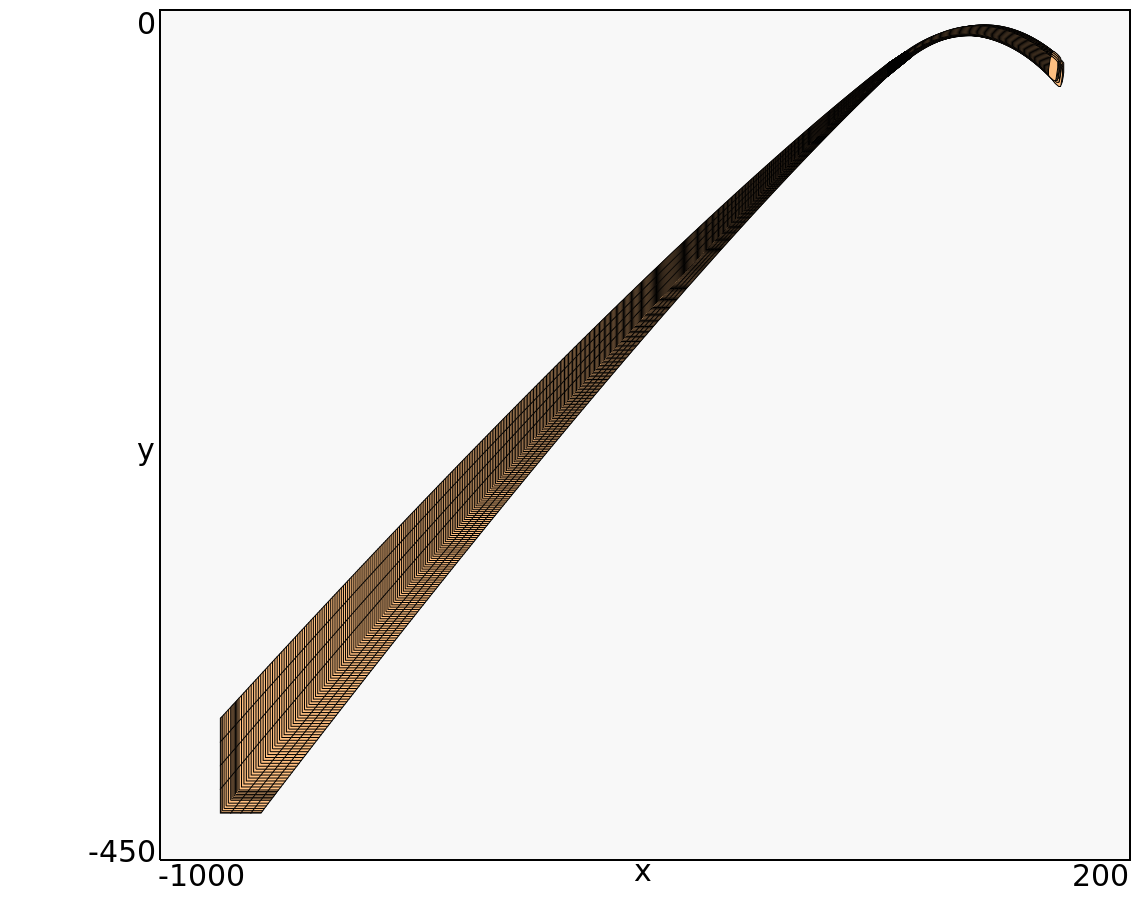
\includegraphics[width=5.5cm, height=5.0cm]{results_Ariadne/spacerendezvous.png}
  \label{fig:spacecraft:ariadne}}
  \hspace{0.2in}
\subfigure[CORA.] 
{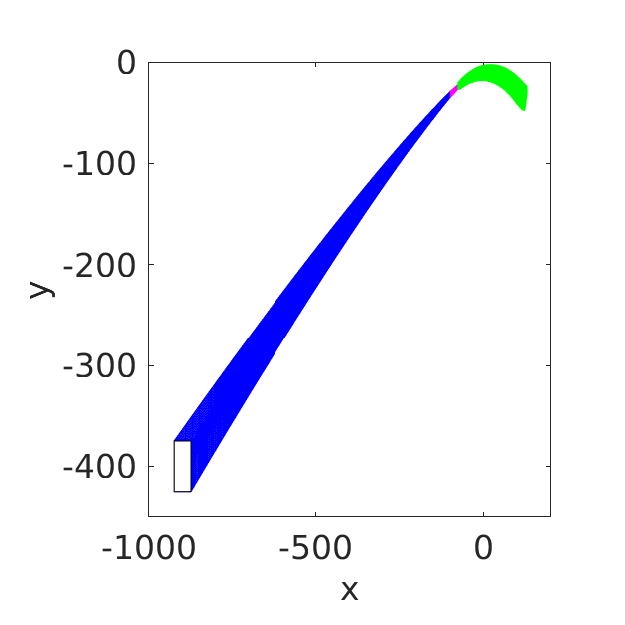
\includegraphics[width=5.5cm, height=5.5cm]{results_CORA/spacecraft_13March2019.eps}
  \label{fig:spacecraft:cora}}
  \hspace{0.2in}
% \subfigure[C2E2.] 
% 	  {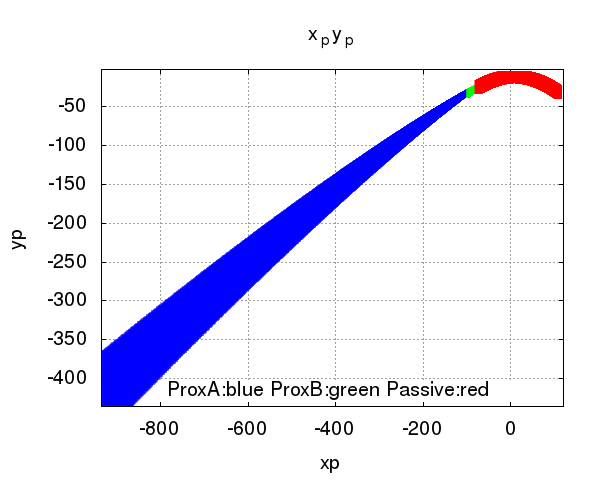
\includegraphics[width=5.5cm, height=5.5cm]{results_C2E2/nln_4d_pass.png}
%   \label{fig:spacecraft:C2E2}}
%   \hspace{0.2in}
  \subfigure[DynIbex.] 
	  {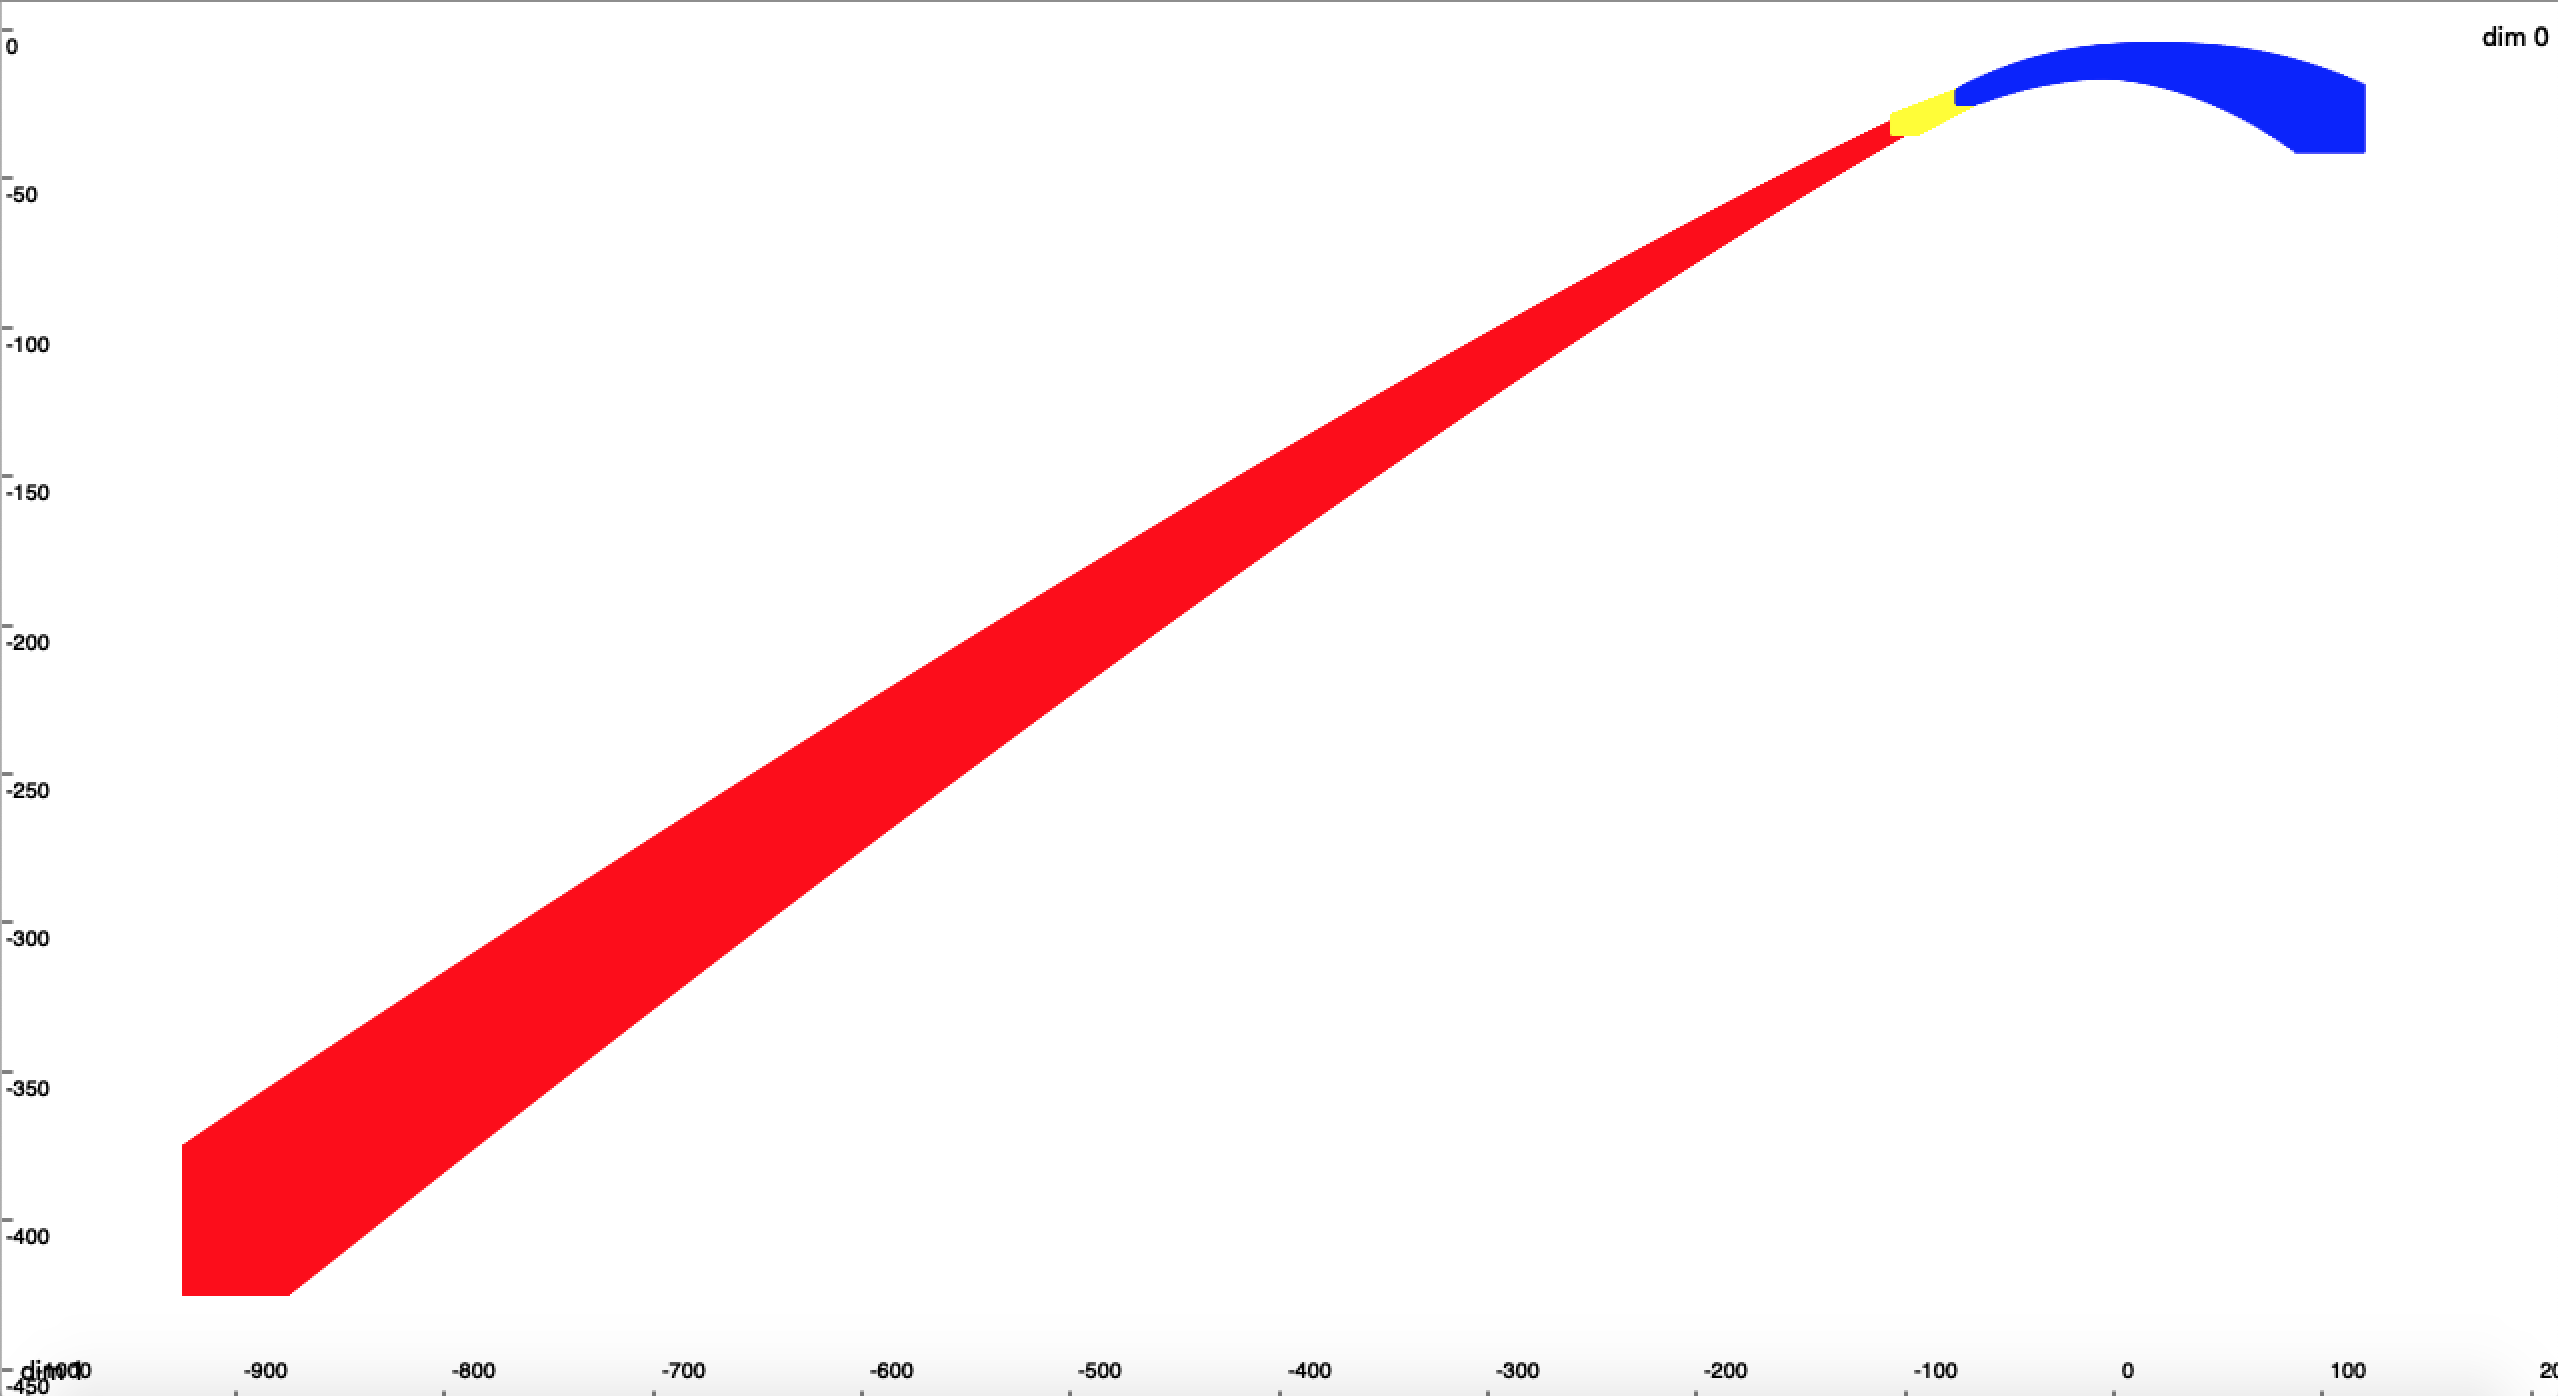
\includegraphics[width=5.5cm, height=5.5cm]{results_DynIbex/space.png}
  \label{fig:spacecraft:dynibex}}
\subfigure[Flow*.] 
	  {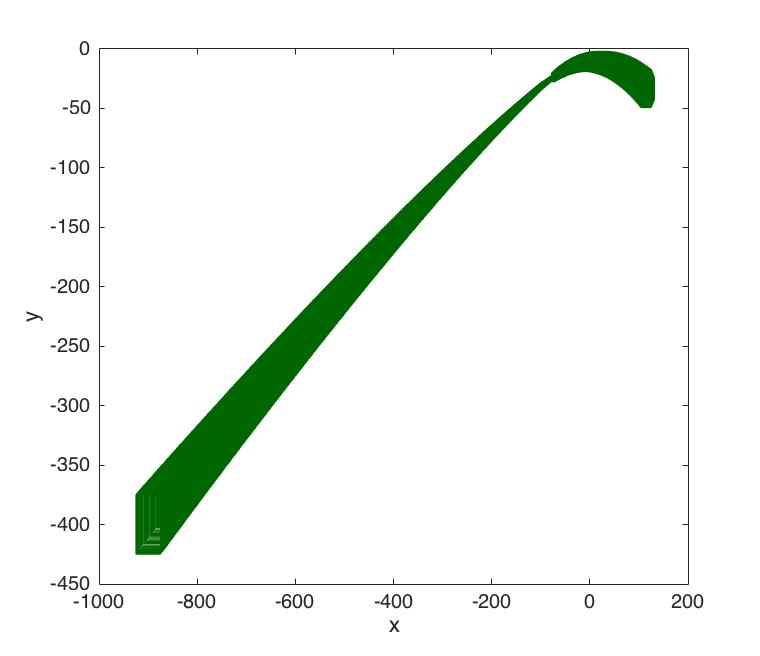
\includegraphics[width=5.5cm, height=5.5cm]{results_flowstar/Space_Rendezvous.png}
  \label{fig:spacecraft:flowstar}}
  \hspace{0.2in}
\subfigure[Isabelle/HOL.] 
	  {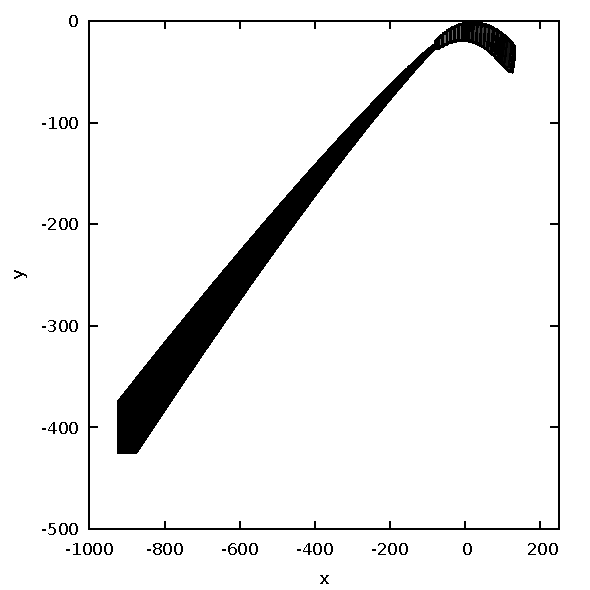
\includegraphics[width=5.5cm, height=5.5cm]{results_Isabelle/out_space.pdf}
  \label{fig:spacecraft:isabelle}}
  \hspace{0.2in}
\caption{Reachable set of the spacecraft position in the $x$-$y$-plane.
CORA, Isabelle/HOL, and DynIbex use different colors to encode different modes of the hybrid system.}
\label{fig:spacecraft}
\end{figure}

\paragraph{Setting for Ariadne.}
The maximum step size used is $1.0$, essentially meaning that we allow the step size to vary widely along evolution: this choice turned out to be preferable in terms of execution time. The maximum temporal order is $4$ and the maximum spacial error enforced for each step equal is $10^{-3}$. A splitting strategy for the initial set is used; the strategy compares the radius of the set with a reference value of $12.0$, in order to split the first two dimensions once and yield a total of $4$ initial subsets.

\paragraph{Setting for CORA.}
CORA was run with a time step size of $0.2$ [min] for the modes \textit{approaching} and \textit{aborting}, and with a time step size of $0.05$ [min] for mode \textit{rendezvous attempt}. The intersections with the guard sets were calculated with the method of Girard, which was introduced in \cite{Girard2008}. In order to find suitable orthogonal directions, the last zonotope that did not intersect the guard set is projected onto the hyperplane that represents the guard set. Then, Principal Component Analysis is applied to the generators of the projected zonotope.

\paragraph{Setting for DynIbex.}
The library does not support hybrid systems automatically but event detection can computed from the reachable tube computed in each mode. Maximum zonotope order is set to $10$, reachability analysis is carried out with an error tolerance of $10^{-6}$ using an explicit Runge-Kutta method of order $2$ (Heun's method). No splitting of the initial state has been performed. The computation of the state-space at a given event time interval $[t_{\min}, t_{\max}]$ is performed by the union of all the boxes of the reachable tube occurring at $[t_{\min}, t_{\max}]$.

\paragraph{Setting for Flow*.}
We use the old version of Flow*. The model can be directly verified by the tool with the following setting for parameters: the TM order is fixed by $5$, the stepsize is adaptively selected in the range from $0.001$ to $0.5$, the remainder estimation is the interval $[-10^{-3},10^{-3}]$ in all dimensions, and the cutoff threshold is $10^{-6}$. Besides, we use the precision $100$. We simply aggregate the intersections after each jump by a box instead of a parallelotope which is more time-costly to compute but more accurate, since it is already sufficient to prove the property.

\paragraph{Setting for Isabelle/HOL.}
Isabelle/HOL does not support hybrid systems automatically.
One can, however, compute the reachable sets for each mode seperately. The intersection with the guard set is computed with the method of Girard~\cite{Girard2008}, simply using axis-aligned orthogonal directions, which results in box enclosures. We verify that the transition to mode \emph{rendezvous attempt} occurs at
$t \in [108.66, 111.71]$,
$x = -100$,
$y \in [-35.04, -28.43]$,
$v_x \in [1.99365, 2.00644]$,
$v_y \in [0.6489, 0.8130]$. Starting from this box, the transition to mode \emph{aborting} occurs at
$t = 120$,
$x \in [-78.02, 71,20]$,
$y \in [-27.34, -20.23]$,
$v_x \in [2.135, 2.341]$,
$v_y \in [0.603, 0.825]$. From there we compute the reachable set until time $t = 200$, which satisfies $y < -1$ [m].
In those computations, maximum zonotope order is set to $50$ and we use absolute and relative error tolerance of $2^{-10}$.

%------------------------------------------------------------------------------

\iffalse
\subsection{Artificial Pancreas}
\label{sec:artificialpancreas}

\subsubsection{Model}

The artificial pancreas benchmark model was introduced in \cite{Chen2017}. It is a hybrid system with nonlinear dynamics. The benchmark models the scenario of an artificial pancreas that automates the delivery of insulin to patients with type-1 diabetes. For the test case, it is assumed that the patient consumes a meal at time $t=0$. It then has to be guaranteed that the controller is able to keep the blood glucose levels at amounts that are not live threatening for the patient. The system states of the benchmark as defined in \cite{Chen2017} (Tab. 2) are the insulin concentration in the remote chamber $X$, the subcutaneous insulin in chamber \#1 $I_{sc1}$ and in chamber \#2 $I_{sc2}$, the glucose concentration in rapidly equilibriating tissues $G_t$, the glucose concentration in plasma $G_p$, the portal vein insulin concentration $I_l$, the insulin in plasma $I_p$, the insulin concentration in chamber \#1 $I_1$, the delayed insulin from chamber \#1 $I_d$ and the subcutaneous glucose concentration $G_s$. 


The differential equations for the artificial pancreas model are given according to \cite{Chen2017}:

\[
\left\{
\begin{array}{lcl}
\dot{X} & = & -0.0278X + 0.0278(18.2129 I_p - 100.25)\\
\dot{I}_{sc1} & = &  -0.0171 * I_{sc1} + 0.97751710655*u_I(t) \\
\dot{I}_{sc2} & = & 0.0152 I_{sc1} - 0.0078 I_{sc2} \\
\dot{G}_t & = & -0.0039 (3.2267+0.0313X) G_t ( 1 - 0.0026 G_t + (2.5097 \times 10^{-6}) G_t^2) \\
& & + 0.0581 G_p - 0.0871 G_t \\
\dot{G}_p & = & 4.7314 - 0.0047 G_p - 0.0121 I_d - 0.0581 G_p + 0.0871 G_t + u_m(t) \\
\dot{I}_l & = & -0.4219 I_l + 0.2250 I_p \\
\dot{I}_p & = & -0.3150 I_p + 0.1545 I_l + 0.0019 I_{sc1} + 0.0078 I_{sc2} \\
\dot{I}_1 & = & -0.0046 ( I_1 - 18.2129 I_p) \\
\dot{I}_d & = & -0.0046 (I_d - I_1 ) \\
\dot{G}_s & = & 0.1 ( 0.5221 G_p - G_s) \\
\end{array}
\right.
\]

The system input $u_m(t) = D u_{m,1}(t)$ is defined by the meal absorption model according to [\cite{Chen2017}, eq. (2)]:

\[
u_{m,1}(t) = \left\{
\begin{array}{lcl}
0 & & t \leq 0\\
1.141 \times 10^{-4} t^2 + 6.134 \times 10^{-6} t & & 0 \leq t \leq 30 \\
5.25 \times 10^{-5} t^2 - 7.468 \times 10^{-3} t + 0.281 & & 30 < t \leq 80 \\
1.245 \times 10^{-7} t^2 - 9.112 \times 10^{-5} t + 2.648 \times 10^{-2} & & 80 < t \leq 360 \\
-6.307 \times 10^{-5} t^2 + 0.0483 t -9.190 & & 360 < t \leq 400 \\
3.553 \times 10^{-6} t^2 - 3.423 \times 10^{-3} t + 0.824 & & 400 < t \leq 500 \\
1.113 \times 10^{-8} t^2 - 1.482 \times 10^{-5} t + 4.9 \times 10^{-3} & & 500 < t \leq 720 \\
0 & & t \geq 720
\end{array}
\right.,
\]
and by the amount of Carbohydrates $D \in [70,80]$ in the meal consumed by the patient. The second system input $u_I(t) = I$ is given by the controller depicted in Fig.~\ref{fig:pancreasController}. One of the main challenges for this benchmark model is the efficient computation of guard intersections in a high dimensional space. 

\begin{figure}[htb]
    \centering	
    \scriptsize
	
      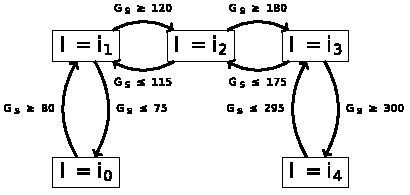
\includegraphics[width=0.6\columnwidth]{./figures/pancreasController.pdf}
      \caption{Control law $u_I(t) = I$ for the artificial pancreas benchmark. The discrete control inputs are defined as $i_0 = 0$, $i_1 = 0.1$, $i_2 = 0.2$, $i_3 = 0.5$ and $i_4 = 1.4$.}
      \label{fig:pancreasController}
\end{figure}


\subsubsection{Specification}

We consider the initial set $X = 0$, $I_{sc1} = 72.42$, $I_{sc2}=141.15$, $G_t=162.45$, $G_p \in [229.824, 268.128]$, $I_l=3.2$, $I_p=5.5$, $I_1 = 100.25$, $I_d=100.25$ and $G_s \in [120,160]$. The amount of Carbohydrates $D \in [70,80]$ in the consumed meal represents an uncertain system input. The unsafe set is $G_s \geq 350$. Further, it is required that $(G_s \leq 300) \land (G_s \geq 250)$ at time $t = 720$. The considered time horizon for the verification is $t \in [0, 720]$. 

\subsubsection{Results}

The results of the reachability computation for the artificial pancreas model are given in Figure~\ref{fig:pancreas} and Table~\ref{tab:compTimes:pancreas}. We give the settings for CORA and Flow* as below.

\begin{table}[h]
	\setlength{\tabcolsep}{4pt}
	\renewcommand{\arraystretch}{1.2}
	\centering
	\caption{Results of the artificial pancreas model. Details of the platforms are described in Section~\ref{sec:machines}.}
	\begin{tabular}[c]{lccc}
	\hline
		 \textbf{tool} & \textbf{computation time in [s]} & \textbf{language} & \textbf{machine} \\
		 \hline
         CORA & $39$ & MATLAB & M$_{\text{CORA}}$ \\
         Flow* & x & C++ & M$_{\text{Flow*}}$ \\
         Isabelle/HOL & x & SML & M$_{\text{Isabelle}}$ \\
		 \hline
	\end{tabular}
	\label{tab:compTimes:pancreas}
\end{table}

\begin{figure}[ht!b]
\centering
\subfigure[CORA.] 
	  {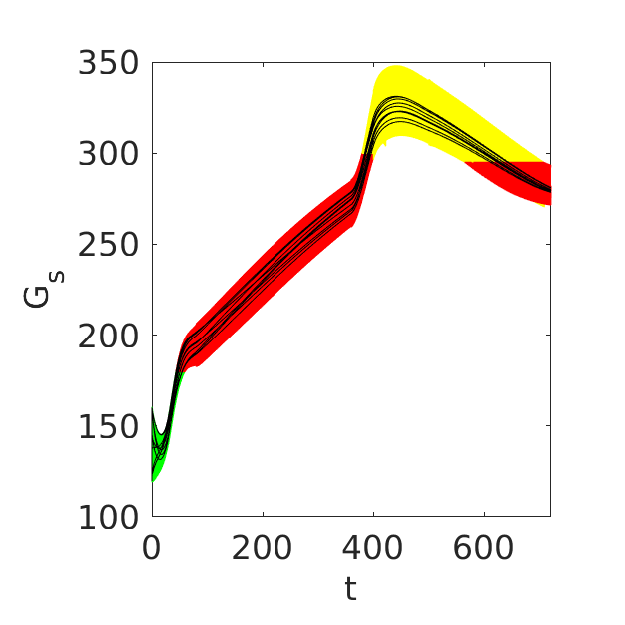
\includegraphics[width=0.45\columnwidth, height=5.5cm]{results_CORA/pancreas_30May2018.eps}
  \label{fig:pancreas:cora}}
  \hspace{0.2in}
\caption{Reachable set of the glucose concentration $G_s$ plotted over time. Simulations are shown in black. The different colors encode different invariant sets of the hybrid system.}
\label{fig:pancreas}
\end{figure}


\paragraph{Setting for CORA.}

CORA uses the step size $0.5$ and the zonotope order $4$. The computation within the invariant sets is carried out using the approach in \cite{Althoff2008c}, which conservatively linearizes the system dynamics for each consecutive time interval by adding the linearization error as an uncertain input. For the calculation of intersections with the guard intersections the approach from \cite{Girard2008} is used. In order to find suitable orthogonal directions, the last zonotope that did not intersect the guard set is projected onto the hyperplane that represents the guard set. Then, Principal Component Analysis is applied to the generators of the projected zonotope.

\paragraph{Setting for Flow*.}





\subsection{Plots}

\subsubsection{Van der Pol Oscillator}

\subsubsection{Laub-Loomis Model}

\textbf{Isabelle Notes:} Reachability Analysis for $W = 0.1$ after splitting the initial set along $x_1$, $x_2$, and $x_3$.

\begin{figure}[ht!b]
\centering
\subfigure[CORA.] 
	  {\includegraphics[width=0.45\columnwidth]{results_CORA/LaubLoomis_30Mar2017.eps}
  \label{fig:laubloomis_easy:cora}}
  \hspace{0.2in}
\subfigure[Isabelle.] 
	  {\includegraphics[width=0.45\columnwidth]{results_Isabelle/laub_time_easy.pdf}
  \label{fig:laubloomis_easy:isabelle}}
\caption{Reachable sets (W=0.01).}
\label{fig:laubloomis}
\end{figure}







\subsection{Quadrotor Model}




\subsection{Computation Times}

The computation times of various tools for the van der Pol benchmark are listed in Tab.~\ref{tab:compTimes:vanderpol}.


\begin{table}[h]
	\setlength{\tabcolsep}{4pt}
	\renewcommand{\arraystretch}{1.2}
	\centering
	\caption{Computation Times of the van der Pol Benchmark.}
	\begin{tabular}[c]{lccccc}
	\hline
		 & \multicolumn{3}{c}{\textbf{computation time in [s]}} & \multicolumn{2}{c}{\textbf{platform}} \\ \cmidrule(l){2-4} \cmidrule(l){5-6}
		 \textbf{tool} & \textbf{van der Pol} & \textbf{Laub ($W=0.01$)} & \textbf{Laub ($W=0.1$)} & $\textbf{language}$ & $\textbf{machine (see  Sec.~\ref{sec:machines})}$ \\ \hline
         CORA & $9$ & $3$ & $63$ & MATLAB & M$_{CORA}$ \\
         Flow* & $2$ & $8$ & $18$ & C++ & M$_{\text{Flow*}}$ \\
         Isabelle & $3$ & $60$ & $2700$ & SML & M$_{Isabelle}$ \\
		 \hline
	\end{tabular}
	\label{tab:compTimes:vanderpol}
\end{table}
\fi

%------------------------------------------------------------------------------
%\section{Discussion}
%\label{sect:discussion}


%------------------------------------------------------------------------------
\section{Conclusion and Outlook}
\label{sect:conclusion}

% From the results of the competition on nonlinear systems, we can see that the techniques handling nonlinear dynamics often require more user-specified parameters than those for linear dynamics. all of the tools have their advantages on some examples, and the applicability of a tool to one example is usually quite sensitive to the computational setting in use. Therefore, it could be a promising direction for coming up with new techniques to find proper settings for a tool and optimize its performance for a given computation task.

% In the next year, we hope that more tools could join the friendly competition and we will also collect more benchmarks which are not only continuous but also hybrid. We will also try to expose the advantages of different tools by examples. The reports of other categories can be found in the proceedings and on the ARCH website:  \href{http://cps-vo.org/group/ARCH}{cps-vo.org/group/ARCH}.
Three tools participated for the first time in the Nonlinear Dynamics category of ARCH-COMP: Ariadne, DynIbex, and JuliaReach. Unfortunately, three tools from last year did not continue to participate: CORA/SX, C2E2, and SymReach.

We always cared about repeatability of the reported results.
This year, we enforced a uniform format for repeatability packages:
All of the tools and benchmarks are made available as Docker~\cite{boettiger2015introduction} containers (on \href{https://gitlab.com/goranf/ARCH-COMP}{gitlab.com/goranf/ARCH-COMP}).
This improves and simplifies reproducibility of our results.

Compared to last year's competition~\cite{ARCH_COMP18}, we made some careful adjustments to the existing benchmark problems to provide a more fine-grained overview of the capabilities of the different tools:
We included a parameter for the stiffness of the van-der-Pol system, added another initial set to the Laub-Loomis problem, and report on the width of final enclosures.

We evaluate this inclusion of additional parameters as a success.
One can see that $\mu$ has a significant influence on the difficulty of the van-der-Pol system for the participating tools, and we might expand more on this influence in future competitions. The additional initial set in the Laub-Loomis problem delineates limitations of the participating tools more precisely.

Triggered by the participation in this competition, individual tools made progress:
%and can now solve benchmarks that were previously out of reach:
\begin{itemize}
\item Flow* entirely updated its module for continuous dynamics, which  shows a much better performance while maintaining the same (or even better) precision.
\item Isabelle/HOL still cannot automatically deal with hybrid systems, but its internals have been refactored significantly. This will simplify automatic reachability analysis for hybrid systems. This refactoring will also help to implement a stand-alone application that parses a standard input file format in the future.
\item Last year, JuliaReach participated only in the AFF category. This competition fostered the \emph{first} collaboration between the two halves of the JuliaReach team. The JuliaReach team evaluates this collaboration as very fruitful and is expecting to participate in next year's edition.

\end{itemize}

%------------------------------------------------------------------------------
\section{Acknowledgments}
\label{sect:acks}


The authors gratefully acknowledge financial support by the European Commission project UnCoVerCPS under grant number 643921. Luis Benet acknowledges the support from PAPIIT grant IG-100819. Alexandre Chapoutot benefited from the support of the “Chair Complex Systems Engineering – Ecole Polytechnique, THALES, DGA, FX, Dassault Aviation, DCNS Research, ENSTA ParisTech, Télécom ParisTech, and Fondation ParisTech”  and he is grateful to Julien Alexandre dit Sandretto for his precious help in the implementation of some examples in DynIbex.

Fabian Immler: This material is based upon work supported by the Air Force Office of Scientific Research under grant number FA9550-18-1-0120. Any opinions, finding, and conclusion or recommendations expressed in this material are those of the author(s) and do not necessarily reflect the views of the United States Air Force.

\appendix
\section{Specification of Used Machines} \label{sec:machines}

\subsection{\texorpdfstring{M$_{\text{Ariadne}}$}{M-Ariadne}} \label{sec:machine:Ariadne}
Virtual machine on VirtualBox 6.0 on macOS 10.14.3 with a single core CPU and 8.0 GB of reserved memory. The operating system of the VM is Ubuntu 18.04.2 LTS. The physical CPU is given as below:
\begin{itemize}
    \item Processor: Intel Core i7-6920HQ CPU @ 2.90GHz x 4 
    \item Average CPU Mark on \url{www.cpubenchmark.net}: 9599 (full), 2019 (single thread)
\end{itemize}
Ariadne currently does not exploit multi-threading.

\subsection{\texorpdfstring{M$_{\text{CORA}}$}{M-CORA}} \label{sec:machine:CORA}

\begin{itemize}
    \item Processor: Intel Core i7-7820HQ CPU @ 2.90GHz x 4 
    \item Memory: 32 GB
    \item Average CPU Mark on \url{www.cpubenchmark.net}: 9409 (full), 2070 (single thread)
\end{itemize}

\subsection{\texorpdfstring{M$_{\text{Flow*}}$}{M-Flow*}} \label{sec:machine:flowstar}
Virtual machine on VMware Workstation 11 with a single core CPU and 4.0 GB memory. The operating systems is Ubuntu 16.04 LTS. The physical CPU is given as below.
\begin{itemize}
 \item Processor: Intel Xeon E3-1245 V3 @ 3.4GHz x 4
 \item Average CPU Mark on \url{www.cpubenchmark.net}: 9545 (full), 2155 (single thread)
\end{itemize}

\subsection{\texorpdfstring{M$_{\text{Isabelle}}$}{M-Isabelle}} \label{sec:machine:isabelle}
\begin{itemize}
 \item Processor: Intel Core i7-8750H CPU @ 2.20GHz x 6
 \item Memory: 16 GB 2666 MHz DDR4
 \item Average CPU Mark on \url{www.cpubenchmark.net}: 12,516 (full), 2368 (single thread)
\end{itemize}

\subsection{\texorpdfstring{M$_{\text{JuliaReach}}$}{M-JuliaReach}} \label{sec:machine:juliareach}
\begin{itemize}
 \item Processor: Intel Core i7-4770HQ CPU @ 2.20GHz x 4
 \item Memory: 16 GB
 \item Average CPU Mark on \url{www.cpubenchmark.net}: 8948 (full), 1893 (single thread)
\end{itemize}

%\subsection{\texorpdfstring{M$_\mathit{SpaceEx}$}{M-SpaceEx}} \label{sec:machine:spaceex}
%\begin{itemize}
%	\item Processor: Intel Core i7-7920HQ CPU @ 3.1GHz x 4
%    \item Memory: 16 GB
%    \item Average CPU Mark on \url{www.cpubenchmark.net}: 10230 (full), 2161 (single thread)
%\end{itemize}

\subsection{\texorpdfstring{M$_{\text{DynIbex}}$}{M-DynIbex}} \label{sec:machine:DynIbex}
\begin{itemize}
 \item Processor: Intel(R) Core(TM) i5-7Y54 CPU @ 1.20GHz x 2
 \item Memory: 8 GB
 \item Average CPU Mark on \url{www.cpubenchmark.net}: 3603 (full), 1379 (single thread)
\end{itemize}


\bibliographystyle{plain}
%\bibliographystyle{alpha}
%\bibliographystyle{unsrt}
%\bibliographystyle{abbrv}
\bibliography{bib/geretti,bib/chen,bib/althoff_other,bib/althoff_own,bib/frehse,bib/immler,bib/c2e2,bib/SymReach,bib/JuliaReach,bib/dynibex}

\end{document}
